\section{Methods}\label{sec:methods}

\cref{sec:intro,sec:background} established that three
independent programs---Manin's $\mathbb{F}_1$-geometry, string theory's
dimensional compactification, and the Hilbert--P\'olya conjecture---converge
on a common geometric need: a dimension that exists topologically but not
algebraically.  The structural correspondence
$\mathbb{F}_1\cong D^1_{\text{compactified}}$, supported by the
Connes--Douglas--Schwarz equivalence, characterizes this dimension as a
degenerate $S^1$ fiber with multiplicative scaling but no additive extension.

This section constructs that dimension explicitly.  The generating mechanism
is the golden ratio~$\golden$ through its defining relation
$\golden^2 = \golden + 1$, which extends the role of $i^2=-1$ from
algebraic ($\mathbb{R}\to\mathbb{C}$) to geometric
($\mathbb{C}\to\Ecube$) dimensional emergence.  From this foundation, the
construction proceeds through a dimensional emergence chain:
\[
  \mathbb{R}^1
    \;\xrightarrow{\times i}\;
  \mathbb{C}^2
    \;\xrightarrow{\times\golden}\;
  \Ecube
    \;\xrightarrow{\text{Wick}}\;
  \mathcal{M}^4
    \;\xrightarrow{\times\sigma}\;
  \mathcal{M}^5_{\mathrm{PCF}}.
\]
Every structural claim is formally verified in Lean~4 (\cref{app:lean}).

% ------------------------------------------------------------------
\subsection{Axiomatic Framework}\label{ssec:axioms}
% ------------------------------------------------------------------

We establish five axioms that define the PCF operator construction.
These axioms emerge from the restrictions identified in~\cref{sec:intro}
(Frobenius, Lawvere, Yanofsky) and provide the foundational constraints that
all subsequent development must satisfy.

\emph{Axiom~1 (Inheritance).}  The operator inherits the axioms
of~$\mathbb{C}$: field structure, completeness, and algebraic closure.

\emph{Axiom~2 (Extension via generators).}  There exist two singular
algebraic generators that extend~$\mathbb{R}$: $i^2=-1$ produces
$\mathbb{R}\to\mathbb{C}$, and $\golden^2=\golden+1$ produces the
geometric coupling $\mathbb{C}\to\Ecube$.

\emph{Axiom~3 (Orthogonal extension).}  There exists a coordinate
$z\in\mathbb{R}$ orthogonal to $(x,y)\cong\mathbb{C}$, coupled by
$z=\golden y$.

\emph{Axiom~4 (Distributed structure).}  The operator factorizes as
$\Omega = P\cdot C\cdot F$, where $P$, $C$, $F$ are complex phasors.
No component ``observes'' itself directly---the self-reference is distributed
among three components, avoiding the prohibited binary cycle that generates
paradoxes (Lawvere--Yanofsky).

\emph{Axiom~5 (Functional fixed point).}  The modulus is constant:
$|\Omega(z,\sigma)|=1/2$ for all $z\in\mathbb{C}$, $\sigma\in\mathbb{R}$.

\begin{Definition}[Axiomatic basis]\label{def:axioms}
The PCF framework rests on the following axioms and definitions:
\begin{align}
  i^2 &= -1,
    \label{eq:i-sq}  \\
  \golden^2 &= \golden + 1,
    \label{eq:phi-sq}  \\
  \mathrm{fib}(0) = 0,\quad
  \mathrm{fib}(1) = 1,\quad
  \mathrm{fib}(n{+}2) &= \mathrm{fib}(n{+}1) + \mathrm{fib}(n),
    \label{eq:fib}  \\
  z &= \golden \cdot y \qquad\text{(golden coupling)},
    \label{eq:golden-coupling}  \\
  \Ecube &= \{(x,\, y,\, \golden y) : x,y\in\mathbb{R}\},
    \label{eq:E3}  \\
  \Omega(z,\sigma) &= P \cdot C \cdot F
    \qquad\text{(tripartite factorization)},
    \label{eq:Omega-PCF}  \\
  |\Omega(z,\sigma)| &= \tfrac{1}{2}.
    \label{eq:modulus-Omega}
\end{align}
\end{Definition}

\begin{Definition}[Component norms]\label{def:component-norms}
The three factors carry canonical norms:
\begin{align}
  \norm{P} &= \frac{1}{\sqrt{3}},
    \label{eq:norm-P}  \\
  \norm{C} &= 1,
    \label{eq:norm-C}  \\
  \norm{F} &= \frac{\sqrt{3}}{2}.
    \label{eq:norm-F}
\end{align}
The product norm satisfies:
\begin{align}
  \norm{\Omega} &= \norm{P}\cdot\norm{C}\cdot\norm{F},
    \label{eq:norm-Omega-product}  \\
  \norm{\Omega} &= \frac{1}{\sqrt{3}} \cdot 1 \cdot \frac{\sqrt{3}}{2}
    = \frac{1}{2}.
    \label{eq:norm-Omega-half}
\end{align}
\end{Definition}

\begin{Definition}[Object norm]\label{def:object-norm}
An \emph{object norm} on a monoidal category $(\cat{C},\otimes,I)$ is a
multiplicative assignment $\norm{\cdot}\colon\ob{\cat{C}}\to\mathbb{R}_{>0}$
satisfying:%
\footnote{This is a monoid homomorphism $(\ob{\cat{C}},\otimes,I)\to(\mathbb{R}_{>0},\times,1)$
on objects, not a functor in the categorical sense (no action on morphisms
is required).  In Lean~4, it is realized as a typeclass \texttt{ObjectNorm}
on any \texttt{MonoidalCategory}.}
\begin{enumerate}[label=(N\arabic*)]
  \item $\norm{X}>0$ for all $X\in\ob{\cat{C}}$,
  \item $\norm{X\otimes Y}=\norm{X}\cdot\norm{Y}$ \quad(multiplicativity),
  \item $\norm{I}=1$ \quad(unit normalization).
\end{enumerate}
\end{Definition}

\begin{Definition}[Contractive category]\label{def:contractive-cat}
A \emph{contractive monoidal category} is a tuple
$(\cat{C},\otimes,I,\norm{\cdot})$ equipped with an object norm such that
there exists a tripartite object $\Omega\cong X_1\otimes X_2\otimes X_3$ with
$\norm{\Omega}<1$.
\end{Definition}


% ------------------------------------------------------------------
\subsection{Third Orthogonal Vector (\texorpdfstring{$\Ecube$}{E3})}\label{ssec:E3}
% ------------------------------------------------------------------

The constraint $z=\golden y$ (Axiom~3) generates a geometric extension
$\mathbb{C}\to\Ecube$ that circumvents Frobenius: no three-dimensional
division algebra exists over~$\mathbb{R}$, but the geometric coupling
operates externally to algebraic structure---as a scaling modulus rather
than a field extension.  The dimensional hierarchy is
$\mathbb{R}^1\xrightarrow{\times i}\mathbb{C}^2\xrightarrow{\times\golden}\Ecube$;
each transition preserves the underlying algebraic structure.

\begin{Proposition}[$\Ecube$ basis]\label{prop:E3-basis}
The space $\Ecube$ (\cref{def:axioms},
\cref{eq:E3}) admits the basis $\{1,\, i,\, \golden\}$.
\end{Proposition}

\begin{proof}
By~\cref{eq:E3}, a general point of $\Ecube$ is $(x,y,\golden y)$ with
$x,y\in\mathbb{R}$.  Writing $z = x + iy\in\mathbb{C}$, the third
coordinate $\golden y = \golden\cdot\mathrm{Im}(z)$ is determined by the
$i$-component and the coupling constant~$\golden$.  The triple
$(1,i,\golden)$ spans~$\Ecube$ over~$\mathbb{R}$ with the constraint that
the third component is $\golden$ times the second; linear independence
follows from the irrationality of~$\golden$.
\end{proof}


% ------------------------------------------------------------------
\subsection{Fibonacci and \texorpdfstring{$\golden$}{phi}}\label{ssec:fibonacci}
% ------------------------------------------------------------------

The golden ratio $\golden$ generates the tripartite structure through
minimal self-reference.  The Fibonacci recurrence
$F_{n+1}=F_n+F_{n-1}$, with
$\lim F_n/F_{n-1}=\golden$, distributes the referential structure across
two predecessors (not one), generating the tripartite decomposition
$\Omega=P\cdot C\cdot F$ as the unique balanced factorization of an
$S_3$-symmetric generator.

We establish $\golden$ as a fixed point through three independent
characterizations, all verified in Lean~4.

The golden ratio~$\golden$ satisfying~\cref{eq:phi-sq} admits two
self-referential characterizations that converge to~$\golden$.

\begin{Lemma}[Continued-fraction fixed point]\label{lem:phi-cf}
\begin{equation}\label{eq:phi-continued-frac}
  \golden = 1 + \frac{1}{\golden}.
\end{equation}
\end{Lemma}

\begin{proof}
From $\golden^2 = \golden + 1$ (\cref{eq:phi-sq}), divide both
sides by $\golden > 0$: $\golden = 1 + 1/\golden$.
\end{proof}

\begin{Lemma}[Nested-radical fixed point]\label{lem:phi-nr}
\begin{equation}\label{eq:phi-nested-radical}
  \golden = \sqrt{1+\golden}.
\end{equation}
\end{Lemma}

\begin{proof}
Since $\golden^2 = \golden + 1 = 1 + \golden$ and $\golden > 0$, taking
positive square roots gives $\golden = \sqrt{1+\golden}$.
\end{proof}

\begin{Proposition}[Golden fixed-point uniqueness]\label{prop:golden-unique}
The equation $x=1+1/x$ for $x>0$ has a unique solution $x=\golden$.
\end{Proposition}

\begin{proof}
The result follows by direct substitution: multiplying by $x>0$ yields the quadratic $x^2 - x - 1 = 0$, which factors as:
\[
  (x - \golden)(x + \golden^{-1}) = 0, \qquad\text{where}\quad \golden^{-1} = \golden - 1.
\]
The root $x = -\golden^{-1} < 0$ violates $x>0$, thus $x = \golden$ is the unique solution.
\end{proof}

The stability of this fixed point is confirmed by the behavior of the continued-fraction sequence.

\begin{Definition}[Continued-fraction sequence]\label{def:cf-seq}
Define $\mathrm{cf}\colon\mathbb{N}\to\mathbb{R}$ recursively:
\begin{equation}\label{eq:cf-def}
  \mathrm{cf}(0)=1, \qquad \mathrm{cf}(n{+}1) = 1 + \frac{1}{\mathrm{cf}(n)}.
\end{equation}
\end{Definition}

\begin{Lemma}[Bounds on $\mathrm{cf}$]\label{lem:cf-bounds}
For all $n \in \mathbb{N}$, the sequence satisfies:
\begin{equation}\label{eq:cf-bounds}
  1 \le \mathrm{cf}(n) \le 2 \qquad\text{and}\qquad
  |\mathrm{cf}(n{+}1)-\mathrm{cf}(n)| \le \golden^{-n}.
\end{equation}
\end{Lemma}

\begin{proof}
We proceed by induction on $n$. For positivity and bounds, $\mathrm{cf}(0)=1$, and $\mathrm{cf}(n)\ge 1$ implies $\mathrm{cf}(n+1)=1+1/\mathrm{cf}(n)\in [1,2]$. For contraction, the map $f(x)=1+1/x$ has $|f'(x)|=x^{-2}\le 1$ on $[1,2]$, and $|f'(\golden)| = \golden^{-2} < 1$. By the Mean Value Theorem:
\[
  |\mathrm{cf}(n+1)-\golden| \le \golden^{-2}|\mathrm{cf}(n)-\golden|,
\]
ensuring geometric decay toward the attractor.
\end{proof}

\begin{Theorem}[Continued fraction converges to $\golden$]%
  \label{thm:cf-converges}
The sequence $\mathrm{cf}(n)$ is Cauchy and $\mathrm{cf}(n)\to\golden$ as $n\to\infty$.
\end{Theorem}

\begin{proof}
Successive differences satisfy $|\mathrm{cf}(n+1)-\mathrm{cf}(n)|\le\golden^{-n}$ by \cref{lem:cf-bounds}. Since $\sum\golden^{-n}$ converges, the sequence is Cauchy. The limit $L$ must satisfy the fixed-point relation $L = 1 + 1/L$, hence $L = \golden$.
\end{proof}

In parallel to the rational approach, the nested radical sequence provides the conjugate geometric characterization.

\begin{Definition}[Nested-radical sequence]\label{def:nr-seq}
Define $\mathrm{nr}\colon\mathbb{N}\to\mathbb{R}$ by:
\begin{equation}\label{eq:nr-def}
  \mathrm{nr}(0)=1, \qquad \mathrm{nr}(n{+}1)=\sqrt{1+\mathrm{nr}(n)}.
\end{equation}
\end{Definition}

\begin{Lemma}[Bounds on $\mathrm{nr}$]\label{lem:nr-bounds}
For all $n \in \mathbb{N}$, the sequence $\mathrm{nr}(n)$ is monotone non-decreasing and bounded: $1 \le \mathrm{nr}(n) \le \golden$.
\end{Lemma}

\begin{proof}
We proceed by induction on $n$. The base case $\mathrm{nr}(0)=1$ satisfies the bounds. If $\mathrm{nr}(n)\le\golden$, then:
\[
  \mathrm{nr}(n+1) = \sqrt{1+\mathrm{nr}(n)} \le \sqrt{1+\golden} = \golden.
\]
For monotonicity, notice that $g(x)=\sqrt{1+x}$ satisfies $g(x) \ge x$ if and only if
\[
  1 + x \ge x^2 \iff x^2 - x - 1 \le 0 \iff x \le \golden.
\]
Since all terms are within $[1, \golden]$, the sequence is non-decreasing.
\end{proof}

\begin{Theorem}[Nested radical converges to $\golden$]%
  \label{thm:nr-converges}
$\mathrm{nr}(n)\to\golden$ as $n\to\infty$.
\end{Theorem}

\begin{proof}
Being bounded and monotone, the sequence must converge to some $L \in [1, \golden]$. The limit relation $L = \sqrt{1+L}$ yields the golden quadratic $L^2 - L - 1 = 0$, whose unique positive root is $\golden$.
\end{proof}

\begin{Remark}
The closed form is $\golden = (1+\sqrt{5})/2$.
\end{Remark}


% ------------------------------------------------------------------
\subsection{Geometric Projection and \texorpdfstring{$\varepsilon_0$}{epsilon_0}}\label{ssec:projection}
% ------------------------------------------------------------------

The orthogonal projection $\pi\colon\Ecube\to\mathbb{C}$ compresses
three-dimensional structure to the complex plane.  The fundamental angular
rotation rate $\varepsilon_0$ and the projection formula encode $|S_3|=6$ and
the effective dimension $d=3$.

\begin{Definition}[PCF projection]\label{def:projection}
\begin{equation}\label{eq:projection-pcf}
  \pi_{\mathrm{PCF}}(a,b,c) = \frac{ab}{c\sqrt{3}}
    \cdot\frac{\pi}{3}.
\end{equation}
\end{Definition}

\begin{Definition}[Fundamental scale]\label{def:epsilon0}
\begin{equation}\label{eq:epsilon0}
  \varepsilon_0 = \frac{\ln\golden}{6\sqrt{3}}.
\end{equation}
\end{Definition}


% ------------------------------------------------------------------
\subsection{Topological Coupling: PCF \texorpdfstring{$\to$}{to} 2D Torus}\label{ssec:torus}
% ------------------------------------------------------------------

The tripartite structure is encoded by the generator matrix
$\OmH = \tfrac{1}{2}\,\mathrm{diag}(1,\omega,\omega^2)$, which is normal
but not Hermitian, encoding the directionality of the P--C--F flow.  Its
three eigenvalues $\lambda_k = \tfrac{1}{2}\omega^k$ satisfy
$|\lambda_k|=1/2$ for all $k$, forming an equilateral triangle inscribed in
the critical circle $|z|=1/2$.  The real parts are
$1/2,\,-1/4,\,-1/4$---only $\lambda_0$ has positive real part.

From the $S_3$ structure, three invariants emerge:
$d=3$ (effective dimension, from $|S_3|=6=3!$),
$\mu=1/2$ (common modulus, from $\norm{P}\cdot\norm{C}\cdot\norm{F}=1/2$),
and $\sigma=d\mu=3/2$ (spectral product).  The provenance of $\sigma=3/2$
is purely geometric:
$\sigma = |{\rm rot}(S_3)|^2/|S_3| = 9/6 = 3/2$.  That the same value
appears as $\zeta(2)/(\pi/3)^2$ reflects the shared numerical
invariants $3$ and $6=3!$ that govern both the $S_3$ structure and the
Basel identity.

\begin{Definition}[Primitive cube root of unity]\label{def:omega-root}
\begin{equation}\label{eq:omega-root}
  \omega = e^{2\pi i/3}.
\end{equation}
\end{Definition}

\begin{Definition}[Operator $\OmH$]\label{def:Omega-hat}
The diagonal matrix and its eigenvalue map:
\begin{align}
  \OmH &= \tfrac{1}{2}\,\mathrm{diag}(1,\,\omega,\,\omega^2),
    \label{eq:Omega-hat-matrix}  \\
  \OmH(k) &= \tfrac{1}{2}\,\omega^k, \qquad k\in\{0,1,2\}.
    \label{eq:Omega-hat-eigenvalues}
\end{align}
\end{Definition}

\begin{figure}[htbp]
\centering
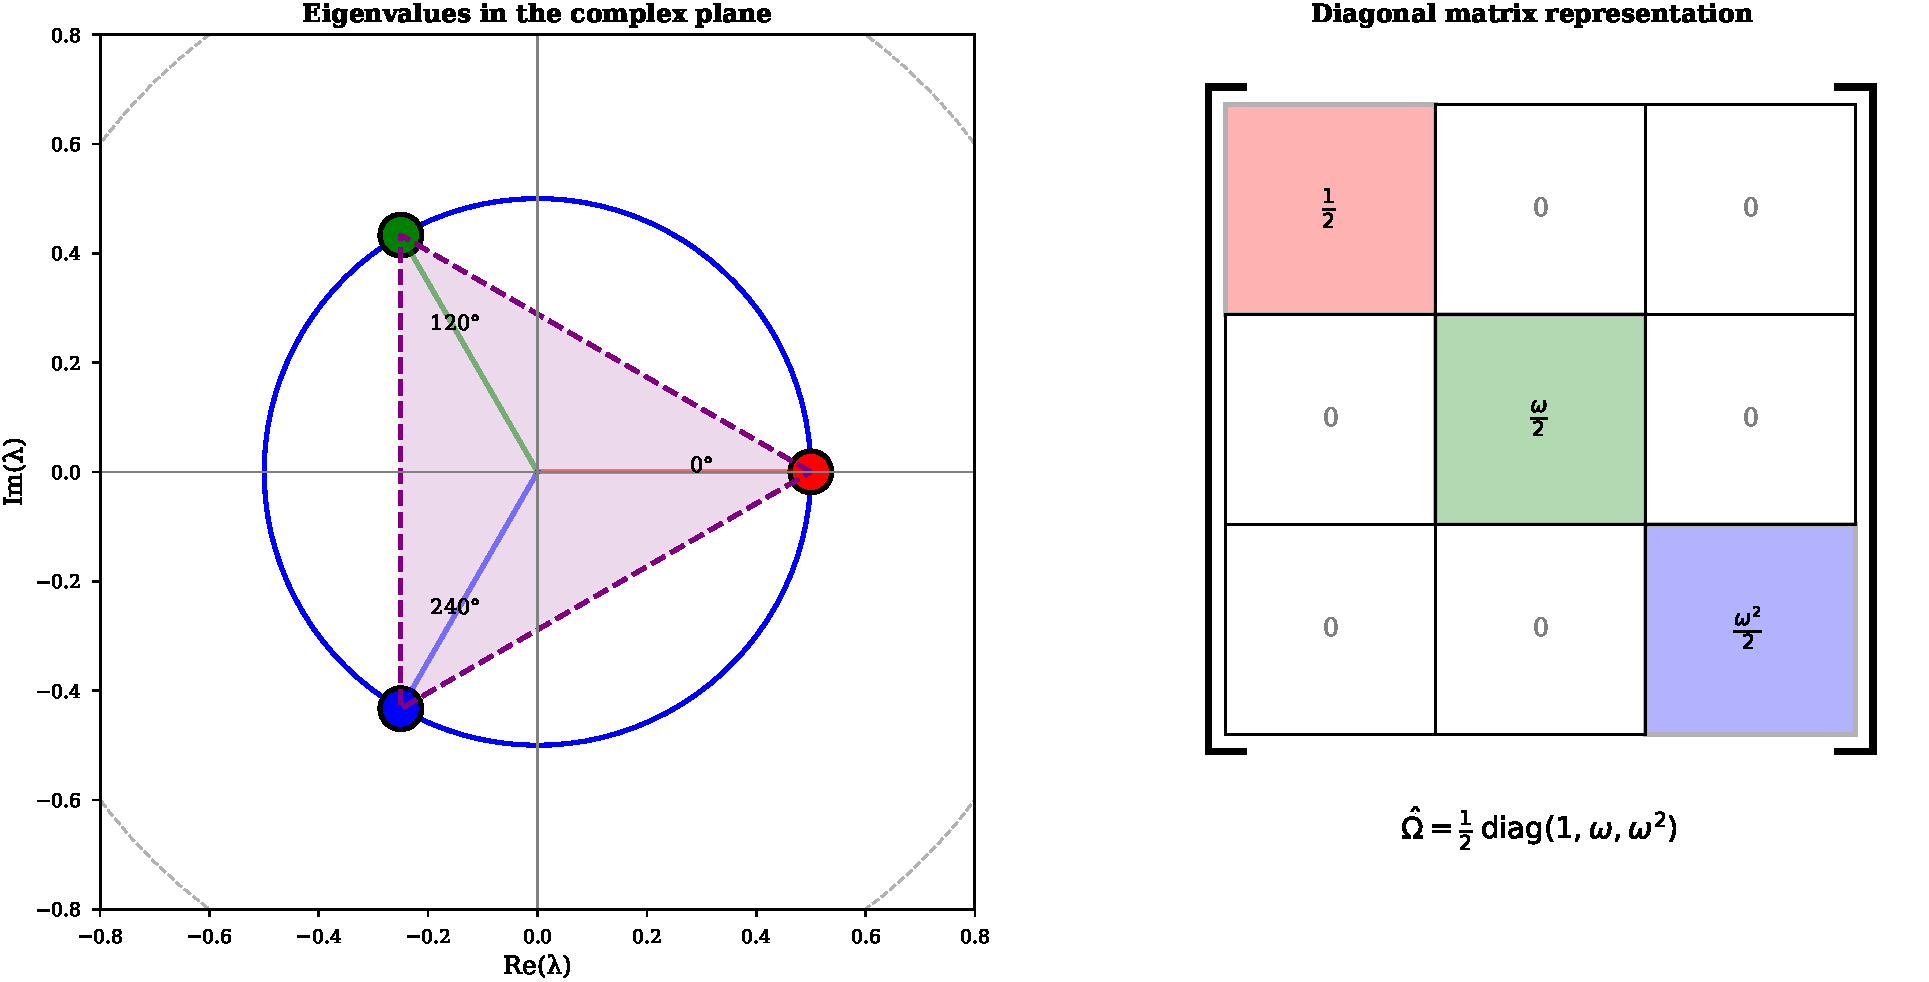
\includegraphics[width=\textwidth]{images/eigenvalues_triangle}
\caption{\textbf{Spectral structure of the PCF operator.}
\emph{Left:} The three eigenvalues $\lambda_k = \tfrac{1}{2}\omega^k$
for $k \in \{0,1,2\}$ inscribed in the
critical circle $|z| = 1/2$. Their $120^\circ$ phase separation encodes
the $S_3$ symmetry of the fundamental triangle.
\emph{Right:} Diagonal matrix representation
$\OmH = \tfrac{1}{2}\operatorname{diag}(1,\omega,\omega^2)$.
The constant magnitude $|\lambda_k| = 1/2$ for all $k$ reflects the
tripartite norm $\norm{P}\cdot\norm{C}\cdot\norm{F} = 1/2$.}
\label{fig:eigenvalues}
\end{figure}


% ------------------------------------------------------------------
\subsection{Lattice Structure and Gauss--Eisenstein Duality}\label{ssec:lattice}
% ------------------------------------------------------------------

The torus $T^2 = \mathbb{C}/(\mathbb{Z}\omega_1+\mathbb{Z}\omega_2)$ with
periods $\omega_1=2\pi/3$ (from $S_3$ symmetry) and $\omega_2=2\pi$ (full
rotation) generates the PCF lattice~$\Lambda_{\mathrm{PCF}}$.  The PCF torus
mediates between the Eisenstein lattice (input, $\mathbb{Z}[\omega]$ from
$120^\circ$ angular separation and $\omega=e^{2\pi i/3}$) and the Gauss
lattice (output, $\mathbb{Z}[i]$ from toroidal closure).  In this dual
structure, the golden ratio provides the bridge: the moduli space
$M_{\mathrm{PCF}}$ is the fundamental domain in which the torus modular
parameter $\tau=\omega_1/\omega_2$ parametrizes the lattice family.

\begin{Definition}[PCF modulus and lattice]\label{def:lattice-pcf}
\begin{align}
  M_{\mathrm{PCF}} &= \frac{6\sqrt{3}\,\pi}{\ln\golden},
    \label{eq:M-pcf}  \\
  \Lambda_{\mathrm{PCF}} &= \langle M_{\mathrm{PCF}},\;
    M_{\mathrm{PCF}}\cdot i\rangle.
    \label{eq:Lambda-pcf}
\end{align}
\end{Definition}

\begin{Definition}[Modular parameter and eigenvalues]\label{def:tau-pcf}
\begin{align}
  \tau_{\mathrm{PCF}} &= i,
    \label{eq:tau-pcf}  \\
  \omega_E &= e^{2\pi i/3}
    \qquad\text{(Eisenstein, coincides with~\cref{eq:omega-root})},
    \label{eq:eisenstein-omega}  \\
  \text{eigenvalues of }\Omega\colon\;&
    k\mapsto \tfrac{1}{2}\,\omega^k
    \qquad\text{(restates~\cref{eq:Omega-hat-eigenvalues})}.
    \label{eq:Omega-eigenvalues-restate}
\end{align}
\end{Definition}
 
\begin{Remark}\label{rmk:gauss-eisenstein-not-new}
These equations are not new definitions, but re-identify the previous ones 
in the Gauss--Eisenstein context.
\end{Remark}

\begin{figure}[htbp]
\centering
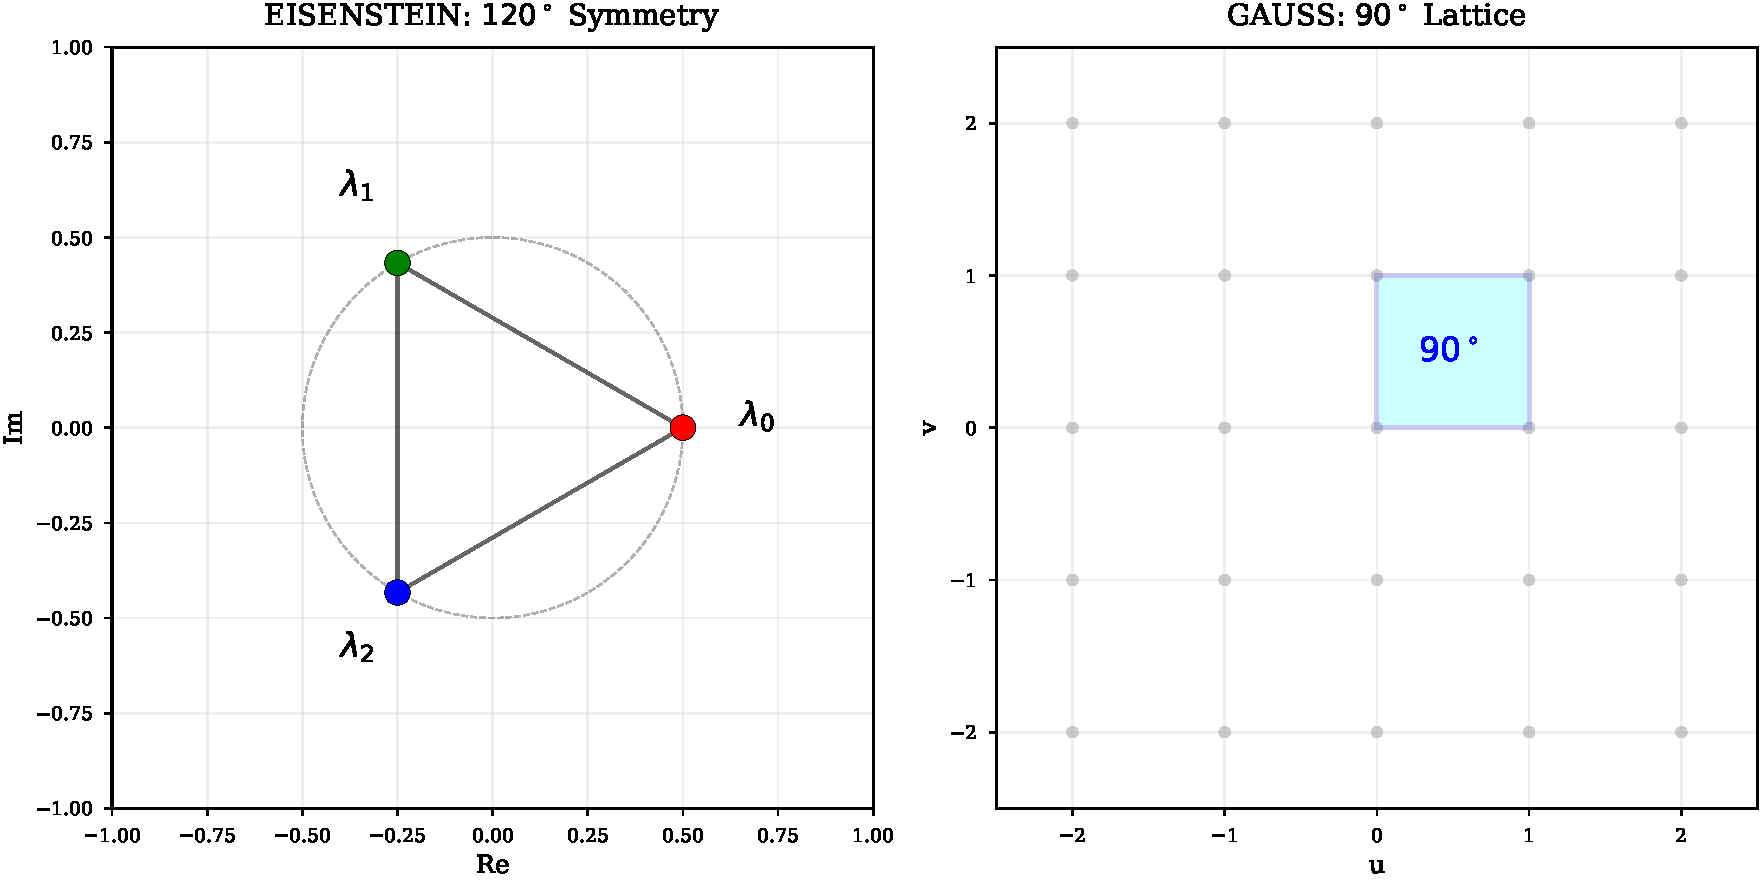
\includegraphics[width=\textwidth]{images/gauss_eisenstein_transition}
\caption{\textbf{Lattice symmetry bridge: Eisenstein to Gauss via $\golden$-coupling.} 
\emph{Left:} The Eisenstein spectrum $(\omega, 120^\circ)$ of the tripartite operator $\OmH$, 
where $|z|=1/2$. \emph{Right:} The Gauss spectrum with modular parameter $\tau = i$ 
and $90^\circ$ fundamental cell. The transition $S_3 \to \mathbb{Z}_4$ 
governs the derivation of the structural parameters $\mu$ and $\sigma$. 
Planar projections (top views) map the circular $120^\circ$ symmetry 
onto the square $90^\circ$ cell, preserving the norm $|\Omega|=1/2$ 
while shifting the algebraic group from $S_3$ to the units of $\mathbb{Z}[i]$.}
\label{fig:gauss-eisenstein}
\end{figure}

\begin{figure}[htbp]
\centering
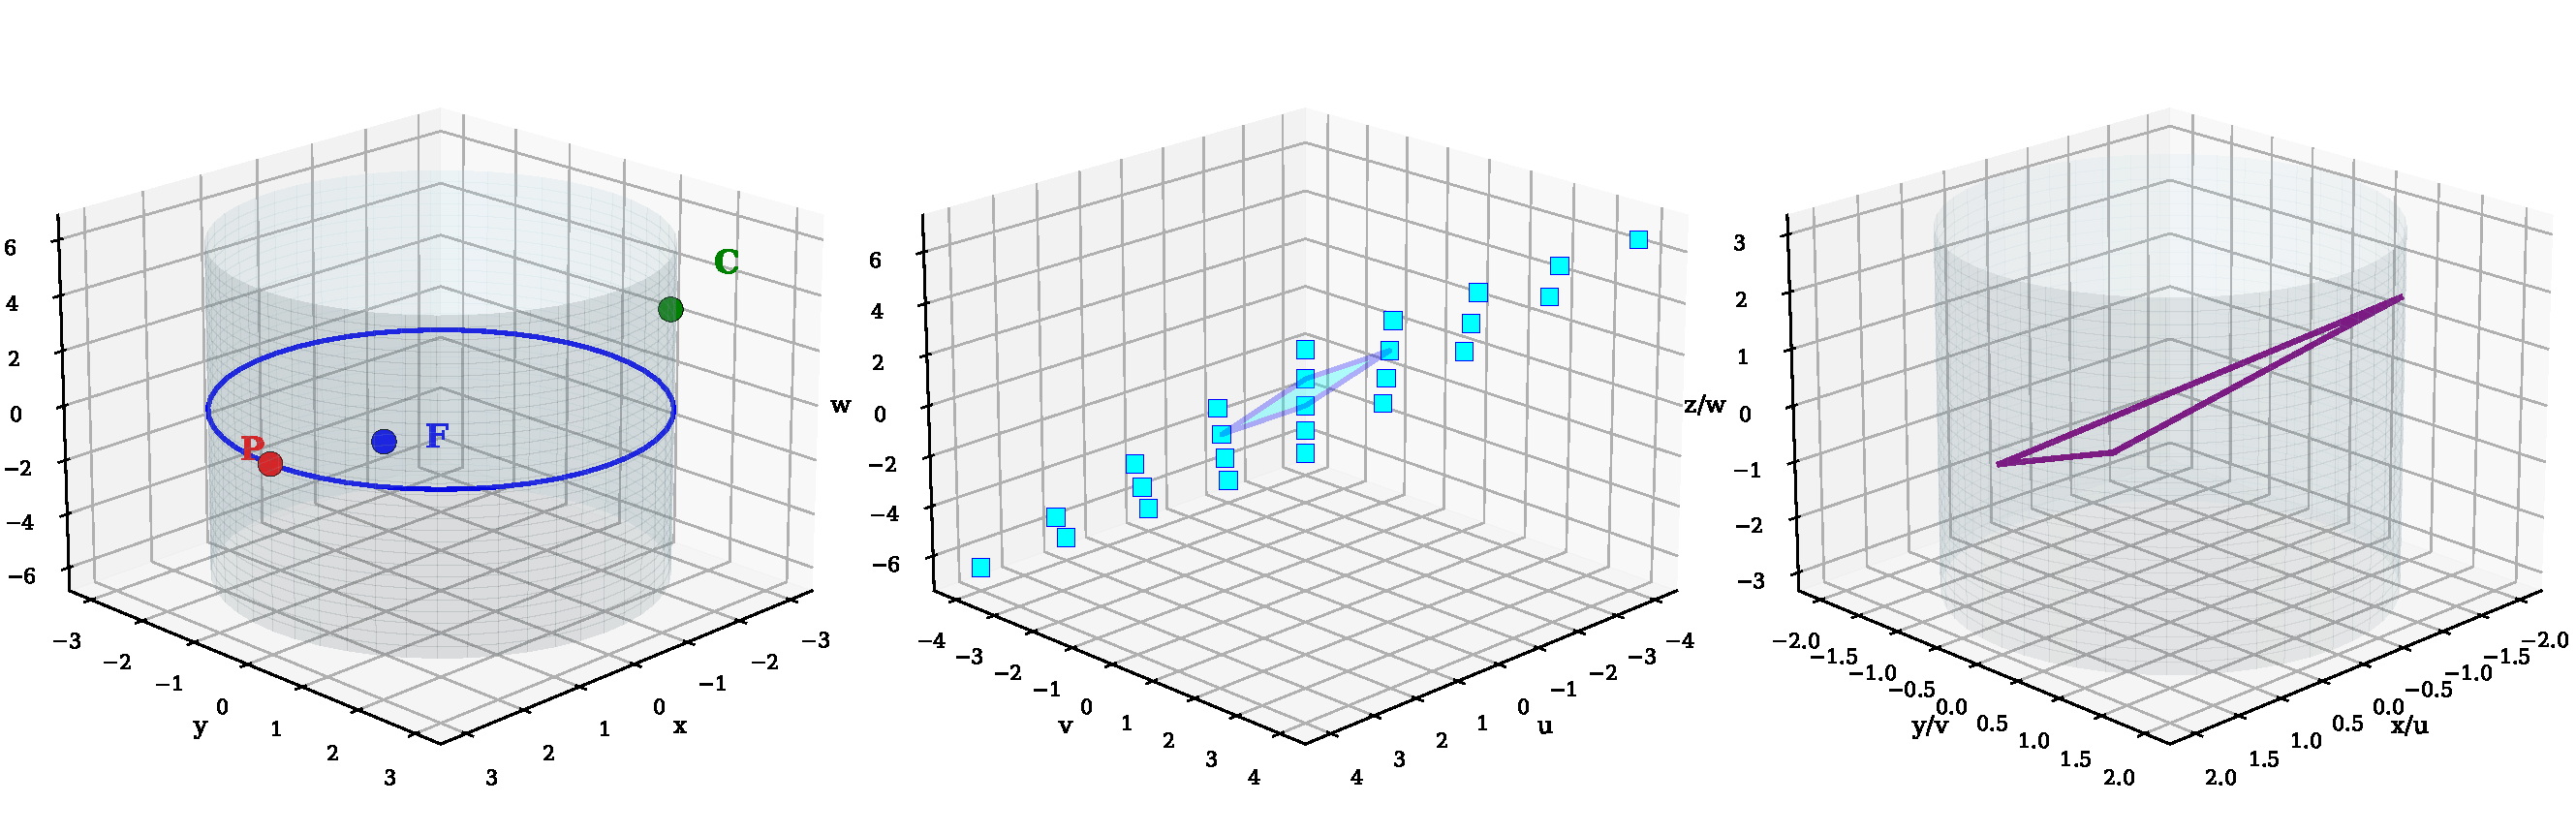
\includegraphics[width=\textwidth]{images/cylinder_lattice_3d}
\caption{\textbf{Geometric embedding of the tripartite state in the PCF lattice.} 
3D spatial realization of the correspondence through the height-to-width 
coupling $z = \golden y$. \emph{Left:} The Eisenstein cylinder $\mathcal{C}_0$ 
hosting the equilateral triangle $P$-$C$-$F$. \emph{Center:} The generated 
orthorhombic lattice $\Lambda_{\mathrm{PCF}}$. \emph{Right:} Spatial 
superposition showing the rigid embedding of the primitive state 
within the lattice structure.}
\label{fig:cylinder-lattice-3d}
\end{figure}



\begin{figure}[htbp]
\centering
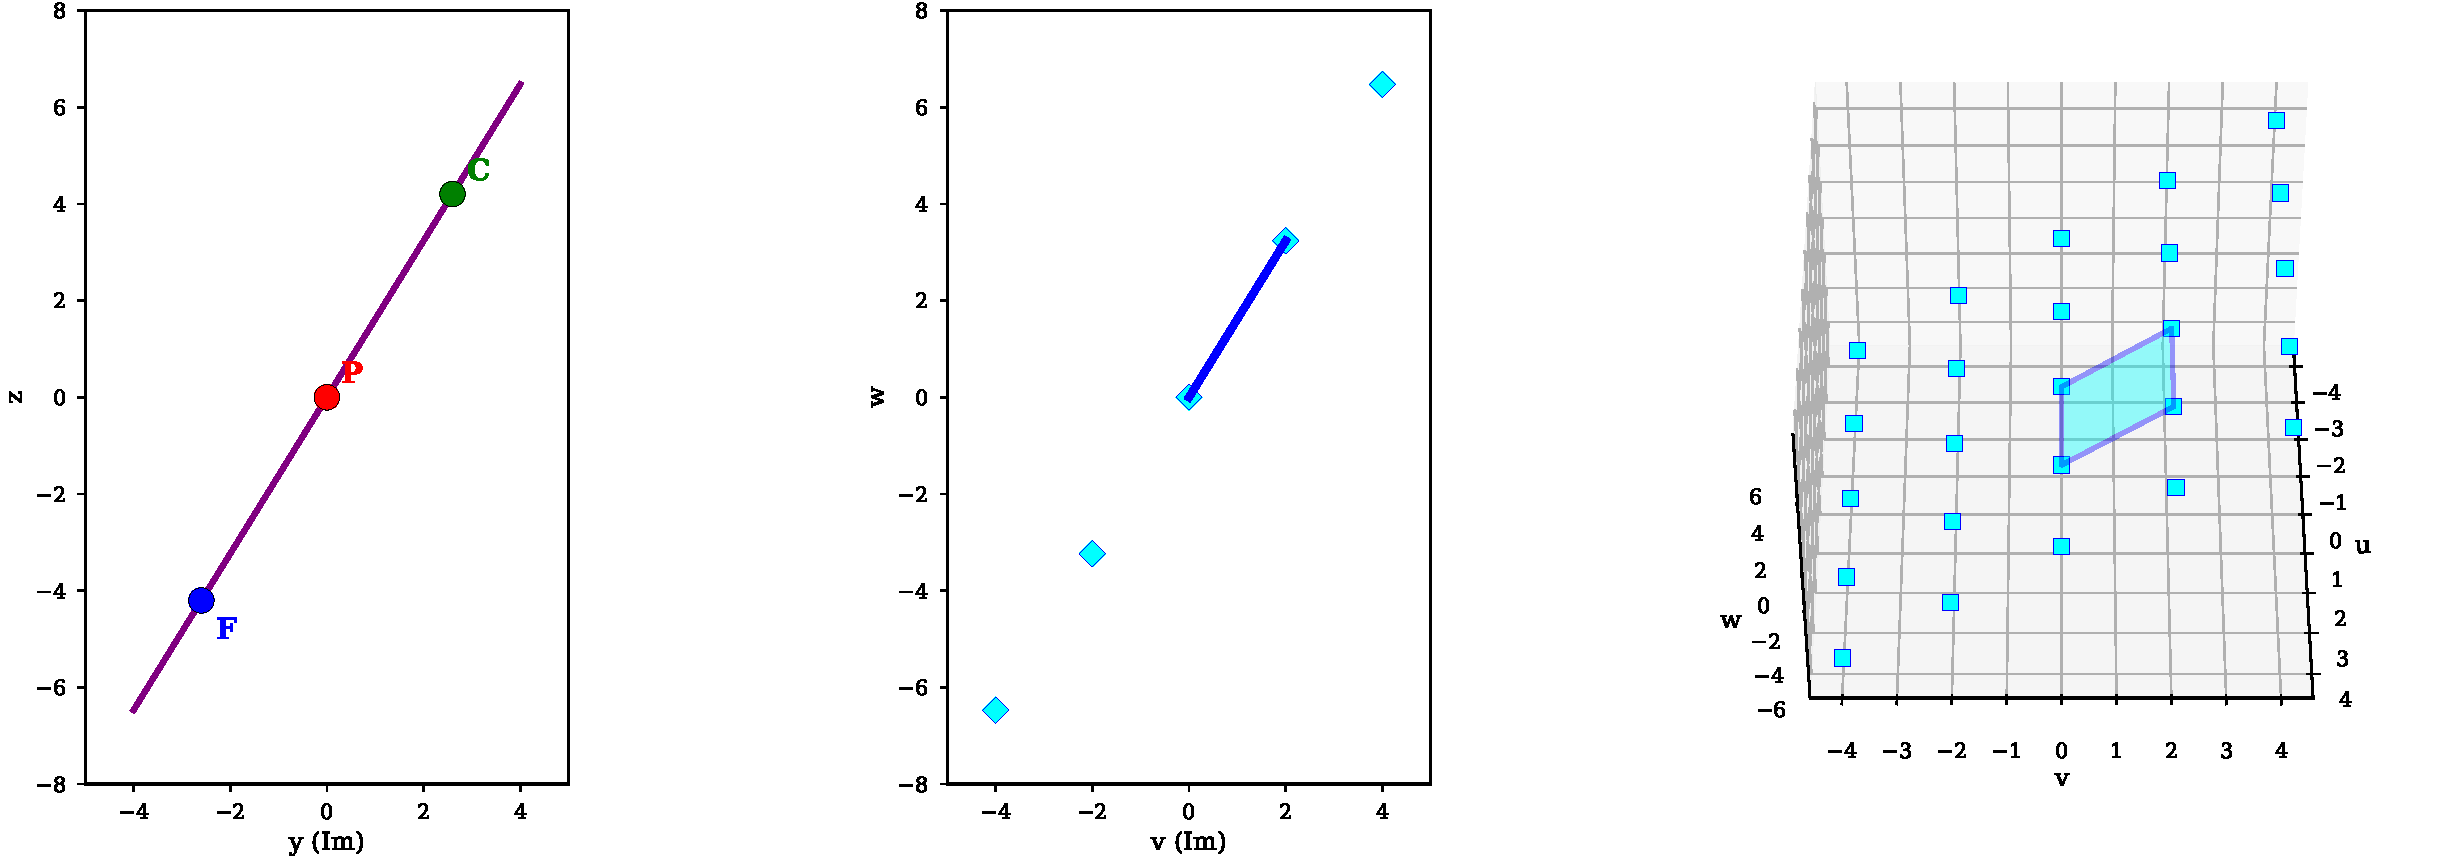
\includegraphics[width=\textwidth]{images/cylinder_lattice_lateral}
\caption{\textbf{Projective constraints and isometric invariants.} 
Multi-perspective views of the symmetry bridge. \emph{Left:} Lateral view 
showing vertex alignment along the slope $\golden$. \emph{Center:} The 
rhombic projection revealing the transition from equilateral to square. 
\emph{Right:} Isometric view of the fundamental unit cell. These 
projections illustrate how the golden ratio $\golden$ mediates 
between the two lattice geometries while preserving the norm $|\Omega| = 1/2$.}
\label{fig:cylinder-lattice-lateral}
\end{figure}


% ------------------------------------------------------------------
\subsection{Self-Similarity and Tower}\label{ssec:tower}
% ------------------------------------------------------------------

The parameter $\sigma\in\mathbb{R}$ generates a tower of
self-similar lattices $\Lambda_\sigma = \golden^\sigma\cdot\Lambda_{\mathrm{PCF}}$,
where each level $\sigma \in \mathbb{Z}$ inherits $|\Omega|=1/2$ and $S_3$ symmetry.  The
self-similarity relation $\varepsilon(\sigma+1)=\golden\cdot\varepsilon(\sigma)$
establishes that angular velocity and spatial scale are bound variables
increasing together through $\golden$-mediation.

\begin{Definition}[Tower parameters]\label{def:tower-params}
\begin{align}
  \lambda_{\log} &= \frac{\ln 2}{\ln\golden},
    \label{eq:lambda-log}  \\
  \varepsilon(\sigma) &= \varepsilon_0\cdot\golden^\sigma,
    \label{eq:epsilon-sigma}  \\
  M_\sigma &= \golden^\sigma \cdot M_{\mathrm{PCF}}.
    \label{eq:M-sigma}
\end{align}
\end{Definition}

\begin{Lemma}[Tower recurrence]\label{lem:tower-recurrence}
\begin{equation}\label{eq:tower-recurrence}
  \varepsilon(\sigma+1) = \golden\cdot\varepsilon(\sigma).
\end{equation}
\end{Lemma}

\begin{proof}
From \cref{def:tower-params}:
$\varepsilon(\sigma+1) = \varepsilon_0\cdot\golden^{\sigma+1}
= \golden\cdot(\varepsilon_0\cdot\golden^\sigma)
= \golden\cdot\varepsilon(\sigma)$.
\end{proof}

\begin{figure}[htbp]
\centering
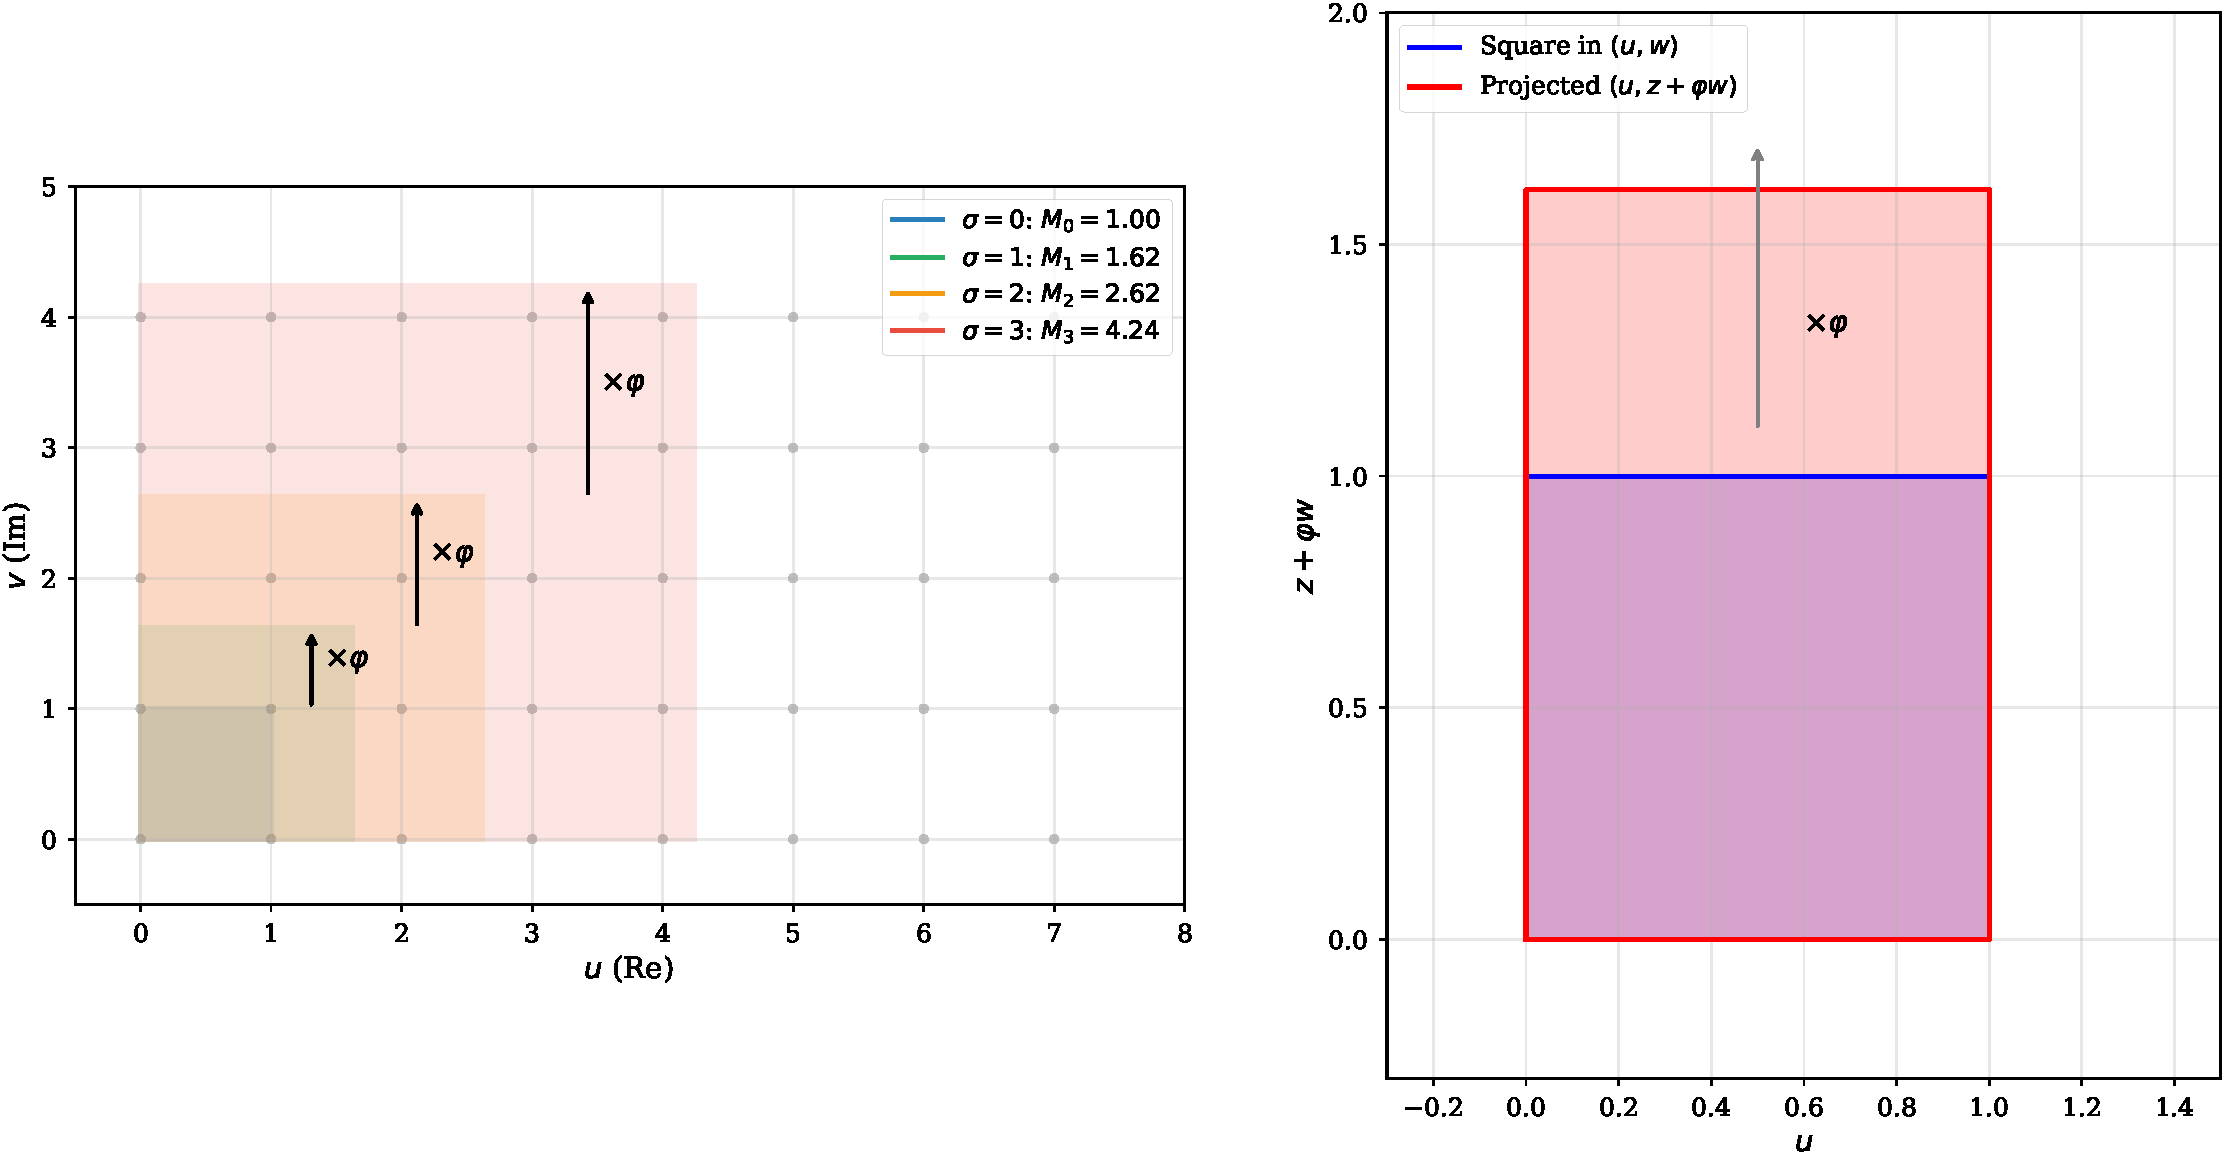
\includegraphics[width=\textwidth]{images/lattice_square_combined}
\caption{\textbf{PCF pentadimensional lattice tower with $\golden^\sigma$ scaling (I).} 
\emph{Top left:} Lattice $\Lambda_{\mathrm{PCF}}$ with fundamental cells 
$M_\sigma = M_{\mathrm{PCF}} \cdot \golden^\sigma$ at levels $\sigma = 0, 1, 2, 3$, 
showing self-similar growth by factor $\golden$ between consecutive levels. 
\emph{Top right:} Golden coupling projection: a square in $(u, w)$ coordinates 
maps to a rectangle in $(u, z + \golden w)$ coordinates, with vertical 
expansion by factor $\golden$ (Axiom~3).}
\label{fig:lattice-combined}
\end{figure}

\begin{figure}[htbp]
\centering
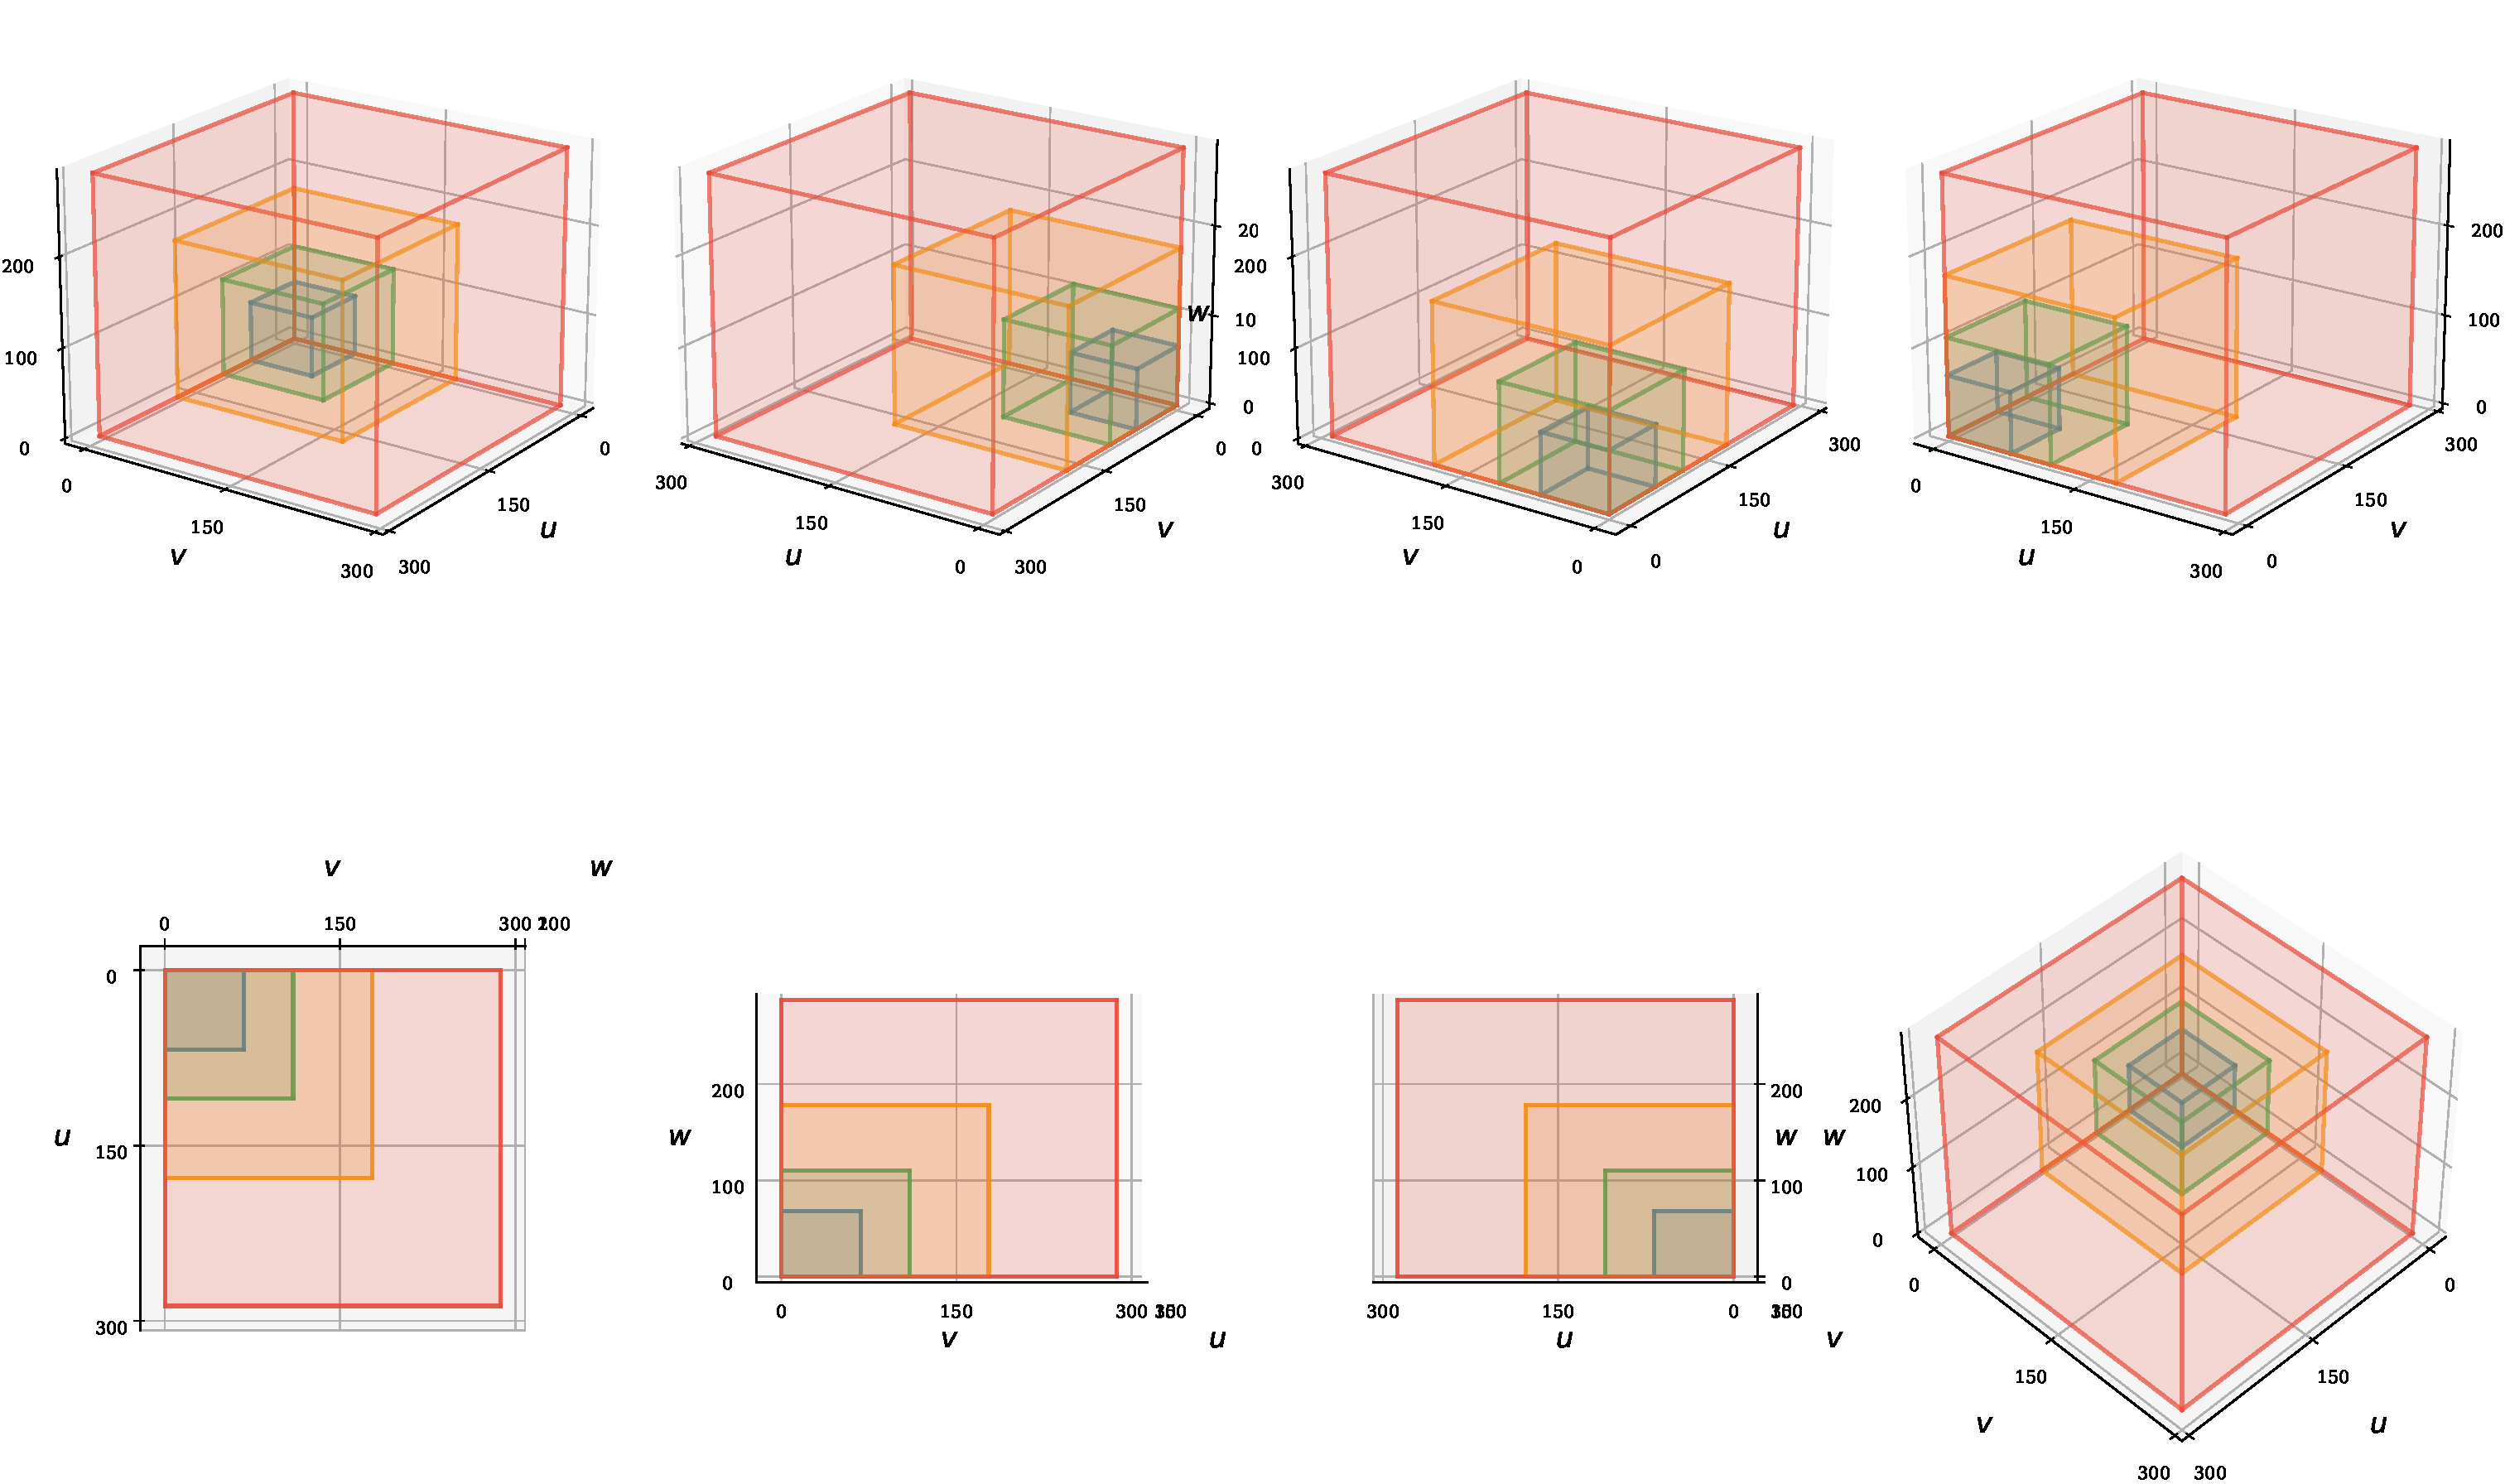
\includegraphics[width=\textwidth]{images/hypercube_views}
\caption{\textbf{PCF pentadimensional lattice tower with $\golden^\sigma$ scaling (II).} 
PCF hypercube in eight complementary views --- four isometric 
perspectives (top row) and four orthogonal projections (bottom row) --- revealing 
nested cubic structures scaling as $\golden^\sigma$. The discrete scale dimension 
$\sigma \in \mathbb{Z}$ parametrizes the pentadimensional structure 
$\mathcal{M}^5_{\mathrm{PCF}} = M^4 \times S^1_\sigma$.}
\label{fig:pentadimensional}
\end{figure}


% ------------------------------------------------------------------
\subsection{Mersenne Connection}\label{ssec:mersenne}
% ------------------------------------------------------------------

The golden tower $\golden^\sigma$ and the Mersenne tower $2^p-1$ are
connected by the logarithmic isomorphism
$\lambda=\ln 2/\ln\golden\approx 1.4404$, with the critical mediator
$|\Omega|=1/2 = \golden^{-\lambda} = 2^{-1}$.  The value $1/2$ is the
unique real number simultaneously satisfying three conditions: it is the
tripartite product $\norm{P}\cdot\norm{C}\cdot\norm{F}$, the tower bridge
$\golden^{-\lambda}=2^{-1}$, and the spectral parameter $\mu_3=2-3/2$
at arity~$3$.

\begin{Definition}[Mersenne and logarithmic bridge]\label{def:mersenne}
\begin{align}
  M(p) &= 2^p - 1,
    \label{eq:mersenne-def}  \\
  \log_\golden(x) &= \frac{\ln x}{\ln\golden}.
    \label{eq:log-phi}
\end{align}
\end{Definition}

\begin{Theorem}[Mersenne bridge]\label{thm:mersenne-bridge}
\begin{equation}\label{eq:mersenne-bridge}
  \golden^{\lambda_{\log}} = 2,
  \qquad\text{where } \lambda_{\log} = \frac{\ln 2}{\ln\golden}
  \approx 1.440
  \;\text{(\cref{eq:lambda-log})}.
\end{equation}
\end{Theorem}

\begin{proof}
The result follows directly by substitution and the application of the natural logarithm exponentiation identity:
\[
  \golden^{\lambda_{\log}}
  = \golden^{\ln 2/\ln\golden}
  = e^{(\ln 2/\ln\golden)\cdot\ln\golden}
  = e^{\ln 2} = 2.
\]
\end{proof}

\begin{Theorem}[Logarithmic correspondence]\label{thm:log-correspondence}
There exists a correspondence $\Phi\colon\sigma\mapsto p_\sigma$ between
levels of the golden tower $R_\sigma = 3\golden^\sigma$ and prime exponents
of Mersenne primes $M_p = 2^p - 1$, determined by:
\begin{equation}\label{eq:log-correspondence}
  \log_\golden(2^{p_\sigma})
    = \sigma\cdot\lambda_{\log} + \log_\golden(3),
\end{equation}
where $\lambda_{\log} = \ln 2/\ln\golden$
(\cref{eq:lambda-log}). Numerical validation yields residuals bounded only by the resolution floor of
double-precision arithmetic ($< 10^{-14}$); this correspondence has been
established across the 51 known Mersenne primes spanning over $25$ million
orders of magnitude.
\end{Theorem}

\begin{proof}
Identifying the tower level $R_\sigma = 3\golden^\sigma$ with the binary prime exponent $2^{p_\sigma}$ yields $\log_\golden(3\golden^\sigma) = \log_\golden(2^{p_\sigma})$. Applying the identity from \cref{thm:mersenne-bridge}, we expand the right-hand side:
\[
  \sigma + \log_\golden(3) = p_\sigma \log_\golden(2) = p_\sigma \lambda_{\log}.
\]
This linear relation defines the correspondence $\sigma\mapsto p_\sigma$. As noted in the theorem, any numerical discrepancy in this formal identity is strictly bounded by the resolution floor of 64-bit computation.
\end{proof}

\begin{Proposition}[Critical mediator]\label{prop:critical-mediator}
The modulus $\norm{\Omega} = 1/2 = 2^{-1}$
(\cref{eq:norm-Omega-half}) is necessary and sufficient for the
golden-Mersenne correspondence~\cref{eq:log-correspondence}: it
simultaneously encodes $S_3$ geometry
($\norm{P}\cdot\norm{C}\cdot\norm{F}=1/2$) and binary coupling
($1/2 = 2^{-1}$), anchoring both bases ($\golden$ and~$2$) to a common
geometric constant.
\end{Proposition}

\begin{proof}
From \cref{thm:mersenne-bridge}, $\golden^{\lambda_{\log}}=2$,
so $2^{-1} = \golden^{-\lambda_{\log}}$.  The tripartite product gives
$\norm{\Omega}=1/2$ (\cref{eq:norm-Omega-half}).  Thus
$\norm{\Omega} = 2^{-1} = \golden^{-\lambda_{\log}}$: the same value
links the $\golden$-tower (through $\golden^{-\lambda_{\log}}$) and the
binary tower (through $2^{-1}$) to the $S_3$ geometry (through the
tripartite norm).  If $\norm{\Omega}\ne 1/2$, the three expressions would
not coincide, breaking the correspondence.
\end{proof}

\begin{Remark}[$d = 3 = M_2$]\label{rmk:d-equals-M2}
The PCF dimension $d=3$ (from $S_3$ symmetry) is itself the first
Mersenne prime: $3 = 2^2 - 1 = M_2$. This reflects the
arithmetic-geometric correspondence: the ternary structure and binary
prime arithmetic are linked through the Mersenne condition $2^p - 1 =
\text{prime}$, with the simplest instance yielding the fundamental
PCF dimension.
\end{Remark}


% ------------------------------------------------------------------
\subsection{Sierpi\'nski Connection}\label{ssec:sierpinski}
% ------------------------------------------------------------------

The IFS with $N=3$ contractions of ratio $r=1/2$ (the three eigenvalue
mappings of~$\OmH$) produces the Sierpi\'nski triangle as attractor.

\begin{Definition}[IFS from $\OmH$ eigenvalues]\label{def:ifs}
Let $v_k = \OmH(k)$ be the eigenvalues~\cref{eq:Omega-hat-eigenvalues}.
The iterated function system is:
\begin{equation}\label{eq:ifs}
  T_k(z) = \tfrac{1}{2}(z - v_k) + v_k, \qquad k\in\{0,1,2\}.
\end{equation}
\end{Definition}


% ------------------------------------------------------------------
\subsection{Hausdorff Dimension}\label{ssec:hausdorff}
% ------------------------------------------------------------------

The Sierpi\'nski attractor encodes the binary--ternary intersection: its
Hausdorff dimension is the ratio of the logarithms of the two arities
($n=3$ and $n=2$) that define the PCF categorical transition.

\begin{Proposition}[Hausdorff dimension of the Sierpi\'nski attractor]%
  \label{prop:hausdorff}
\begin{equation}\label{eq:hausdorff-dim}
  \dim_H = \frac{\ln 3}{\ln 2},
  \qquad\text{satisfying}\quad
  2^{\dim_H} = 3.
\end{equation}
\end{Proposition}

\begin{proof}
The IFS (\cref{def:ifs}) has $N=3$ contractions, each with
ratio $r=1/2$ (since $|\OmH(k)|=1/2$ for all $k$).  By Moran's equation
for self-similar IFS with open set condition,
$\sum_{k=1}^N r_k^d = 1$, i.e., $3\cdot(1/2)^d = 1$, giving
$d = \ln 3/\ln 2$, the Hausdorff dimension of the Sierpi\'nski triangle~\cite{mandelbrot82}. Equivalently, $2^d = 3$, encoding the
binary-to-ternary transition.
\end{proof}


% ------------------------------------------------------------------
\subsection{Moduli--Function Duality and Pentadimensional Synthesis}%
  \label{ssec:synthesis}
% ------------------------------------------------------------------

\begin{Definition}[$\Ecube$ point structure]\label{def:E3-point}
An $\Ecube$-point is a triple $(x,y,\golden y)\in\Ecube$
(cf.~\cref{eq:E3}), with projection:
\begin{equation}\label{eq:proj-E3-to-C}
  \pi\colon \Ecube\to\mathbb{C}, \qquad
  (x,y,\golden y)\mapsto x + iy.
\end{equation}
\end{Definition}

\begin{Proposition}[Certainty principle]\label{prop:certainty}
Let $\varepsilon_0 = \ln\golden/(6\sqrt{3})$ be the base angular rotation
rate of the golden tower (\cref{def:epsilon0}), and
$M_{\mathrm{PCF}} = 6\sqrt{3}\,\pi/\ln\golden$ the spatial period of the
PCF torus (\cref{def:lattice-pcf}).  Then
\begin{equation}\label{eq:certainty-principle}
  \varepsilon_0 \cdot M_{\mathrm{PCF}} = \pi:
\end{equation}
one traversal of the fundamental domain accumulates exactly $\pi$~radians
of phase---a half-turn.  At tower level~$\sigma$, the angular rate
$\varepsilon(\sigma)=\varepsilon_0\golden^\sigma$ grows while the conjugate
wavelength $\pi/\varepsilon(\sigma) = M_{\mathrm{PCF}}\cdot\golden^{-\sigma}$
contracts, their product remaining~$\pi$.
\end{Proposition}

\begin{proof}
Direct computation:
\[
  \varepsilon_0\cdot M_{\mathrm{PCF}}
  = \frac{\ln\golden}{6\sqrt{3}}
    \cdot\frac{6\sqrt{3}\,\pi}{\ln\golden}
  = \pi.
\]
\end{proof}

\begin{Remark}[Geometric content and role within PCF]\label{rem:certainty-content}
The algebraic cancellation in the proof conceals a structural identity
among three geometries.  The numerator of~$\varepsilon_0$ is
$\ln\golden$---the exponential growth rate determined by the
pentagon ($\golden^2=\golden+1$); its denominator $6\sqrt{3}$ encodes
$|S_3|=6$ and the height factor~$\sqrt{3}$ of the equilateral
triangle.  In~$M_{\mathrm{PCF}}$ these roles invert:
$6\sqrt{3}\,\pi$ in the numerator couples triangle geometry to the
circle, while $\ln\golden$ in the denominator supplies the pentagonal
scale.  The product~$\pi$ is therefore not a cancellation artifact
but the \emph{circle emerging from the coupling of triangle and
pentagon}: the torus period and the angular rate are reciprocal
precisely because both are determined by the same two polygonal
inputs, with $\pi$ as their sole common output.

The product equals $\pi$---a half-turn---rather than $2\pi$ because
the tripartite norm $|\Omega|=1/2$
(\cref{eq:norm-Omega-half}) contracts a full $S_3$ rotation
($3\times 2\pi/3=2\pi$) by the factor~$1/2$: one traversal of the
fundamental domain reaches the antipodal point, not the starting
point.  Categorically, this is the geometric expression of the
anti-self-reference mechanism: a full turn ($2\pi$) would implement
$f(f)$---the diagonal self-application that Lawvere's theorem
prohibits (\cref{sssec:lawvere})---while a half-turn implements
distributed passage $f\circ g\circ h$ that does not close.

The identity is a \emph{self-consistency relation with zero free
parameters}: $\golden$, $|S_3|$, $\sqrt{3}$, and $\pi$ are all
geometrically determined, and no Hamiltonian, Virasoro algebra, or
external dynamical input enters.  This addresses exactly the
constructional circularity identified in~\cref{ssec:polya-hist}:
the P\'olya operator cannot be defined from its own spectrum, yet
every prior program requires a presupposed dynamical operator to
generate spectral evolution.  PCF derives the spectral constraint
instead from the mutual determination of Eisenstein geometry
($\varepsilon_0$: pentagon over triangle) on the input side and
Gaussian geometry ($M_{\mathrm{PCF}}$: the square torus
$\Lambda_{\mathrm{PCF}} = \mathbb{Z}M\oplus\mathbb{Z}Mi$ with
$\tau_{\mathrm{PCF}}=i$, \cref{def:tau-pcf}) on the
output side.

The pentagonal ingredient $\ln\golden$ in $\varepsilon_0$ connects
forward to the construction of the operator: the golden ratio governs
the cyclotomic tower
$\Phi_5\to\Phi_{10}\to\Phi_{20}$
(\cref{prop:cyclotomic}) and the Golden Prime
classification $G(p)\in\{\pm\golden,\pm\golden^{-1}\}$
(\cref{thm:golden-prime-classes}), through which~$\golden$
organizes the prime residues that the operator must encode.

Finally, the Mersenne connection (\cref{ssec:mersenne}) is a
direct consequence: combining $\varepsilon_0\cdot M_{\mathrm{PCF}}=\pi$
with the bridge $\golden^{\lambda_{\log}}=2$
(\cref{thm:mersenne-bridge}) yields
$|\Omega|=1/2=2^{-1}=\golden^{-\lambda_{\log}}$---the unique value
anchoring the golden and binary towers to the same geometric point.
\end{Remark}

\begin{Corollary}[Critical dimensions]\label{cor:critical-dims}
The PCF architecture is structured across five critical dimensions mapping to the Fibonacci-graded introduction of algebraic generators and the structural unfolding of the spectral manifold $\mathcal{M}^5_{\mathrm{PCF}}$.

\begin{center}
\footnotesize
\begin{tabular}{@{}cllll@{}}
\toprule
$d$ & Manifold & Generator & Lean witness & Role \\
\midrule
1 & $\mathbb{R}$ & --- & $\mathbb{R}$ & Radial magnitude \\
2 & $\mathbb{C}$ & $i^2=-1$ & $\hat\Omega:\texttt{Fin\,3}\!\to\!\mathbb{C}$ & Gaussian closure \\
3 & $E_{\phi}$ & $z = \golden y$ & $|\Ztwenty|\!=\!8$ & Frobenius circumvented \\
4 & $\mathcal{M}^4$ & Wick factor & $\mu_2/\mu_3 = 2$ & $S^1$ velocity encoding \\
5 & $\mathcal{M}^5_{\mathrm{PCF}}$ & $\sigma$-tower & $\lambda_{\alpha}=20$ & $H_5$ unfolding \\
\bottomrule
\end{tabular}
\end{center}
The dimensions introducing new algebraic generators follow the Fibonacci subsequence $\{1,2,3,5\}$, with dimension $d=4$ representing the temporal coordinate.
\end{Corollary}

\begin{proof}
The dimensional architecture of $\mathcal{M}^5_{\mathrm{PCF}}$ is established as a rigid deductive chain in Lean 4, integrating algebraic extensions, topological obstructions, and combinatorial scaffolding:
\begin{enumerate}
    \item \textbf{Algebraic Extensions ($d=1,2,3$):} The subsequence $\{1,2,3,5\}$ marks the Fibonacci-graded introduction of new generators ($i$, $\golden$, and the $\sigma$-tower). Starting from $\mathbb{R}$ ($d=1$) and the Gaussian closure via $i^2=-1$ (\texttt{i\_const}, $d=2$), the third dimension introduces $z = \golden y$ (Axiom~3). This circumvents the Frobenius--Hurwitz obstruction (\cref{sssec:frobenius}) geometrically, not algebraically via $\mathbb{H}$, which is formalized in Lean via the \texttt{arity\_unique} theorem (proven unique via \texttt{linarith} by bounding $\mu_n$ between 0 and 1).
    \item \textbf{Topological Closure ($d=4,5$):} Dimension $d=4$ is the Wick-rotated temporal coordinate whose content is the angular velocity of \cref{prop:certainty}. The construction reaches completion at $d=5$ through the compactification of the tower parameter into $S^1_\sigma$. The half-turn $\varepsilon_0 \cdot M_{\mathrm{PCF}} = \pi$ implies that $S^1_\sigma$ does not close ($\pi \neq 2\pi$), encoding the anti-self-reference obstruction topologically. This stability is secured by the \texttt{no\_diagonal\_tower} theorem, which employs Lawvere's "no-diagonal" argument to prevent categorical retraction.
    \item \textbf{Combinatorial Scaffolding ($H_3$ and $H_5$):} The hypercube $H_k = \{0,1\}^k$ is fixed by the tower's binary contraction factor $\mu_2/\mu_3 = 2$ (\texttt{contraction\_factor}) and the arity uniqueness $n=3$ (\cref{thm:arity-unique}). Their conjunction yields $2^3=8$ vertices. The sextuple convergence (\cref{prop:sextuple-8}) confirms that no other value is compatible: $|H_3|$, $\varphi(20)$, $|\Ztwenty|$, the octants of $\mathbb{R}^3$, $\beta_0^{-1}$, and $|\mathbb{Z}_2\times\mathbb{Z}_4|$ all equal $8$ independently (verified via \texttt{decide} on \texttt{ZtwentyStar\_card}). At $d=5$, binary branching in pentagonal axes produces $H_5 = \{0,1\}^5$ (\cref{thm:hypercube}). Since $\binom{5}{3}=10$, $H_5$ contains 10 orientations of $H_3$, each with $2^2=4$ translates, yielding $40$ oriented copies of the $8$-vertex cube (\cref{prop:pentagonal-planes}).
\end{enumerate}
These embedded cubes constitute the discrete spectral scaffolding from which the operator parameters $\beta_0 = 1/|H_3|$, $\lambda = |H_2|\times 5 = 20$, and $\alpha_0 = \sigma_3 - \mu_3/\lambda$ are derived. The manifold $\mathcal{M}^5_{\mathrm{PCF}}$ provides the continuous envelope for this dual spectrum.
\end{proof}

\textbf{Comparative synthesis.}
The following table situates PCF among four programs that share the tower
pattern:

\begin{center}
\small
\begin{tabular}{@{}lcccc@{}}
\toprule
 & \textbf{Manin/$\mathbb{F}_1$} & \textbf{String/Virasoro}
 & \textbf{Tarski/Types} & \textbf{PCF} \\
\midrule
Tower mechanism & $\psi^k$ (alg.) & $L_n$ (Virasoro)
  & Universes & $\golden^\sigma$ (geom.) \\
Presupposes $H$? & No (lacks it) & Yes ($L_0{+}\bar{L}_0$)
  & N/A & No \\
Frobenius & Obstructed & Circumvented
  & N/A & Circumvented \\
Self-ref.\ control & None & None & By fiat & $\norm{\Omega}<1$ \\
Decidable fragment & No & No & Yes & Yes \\
Lean formalized & No & No & Partial & Yes \\
\bottomrule
\end{tabular}
\end{center}

The ring $\Rpcf = \mathbb{Z}[\golden,\golden^{-1},\tfrac{1}{2}]$ admits a
$\Lambda$-ring structure with Frobenius lifts $\psi_p(\golden)=\golden^p$,
constituting $\mathbb{F}_1$-descent data in the sense of Borger.  The PCF
tower $\norm{\Omega}_k = (1/2)^{2^k}$ generates dimensional structure by
categorical contraction, not Hamiltonian dynamics---paralleling
Huerta--Schreiber's derivation of the dimensional tower from the superpoint
$\mathbb{R}^{0|1}$ by successive maximal invariant central extensions.
Russell's prohibition $X\in X$ and Tarski's decidable geometry both find
their resolution in the metric condition $\norm{\Omega}=1/2<1$ (No-Diagonal
Theorem, \cref{ssec:CM-cat}).  The arithmetic engine $\Ztwenty$ operates
entirely within the decidable multiplicative fragment; the hypercube count
$|H_3| = 2^3 = 8 = |\Ztwenty|$ links combinatorial and group-theoretic
structure.
Implications are developed in~\cref{sec:discussion}.


% ------------------------------------------------------------------
\subsection{Construction of the Operator \texorpdfstring{$T^*$}{T*}}\label{ssec:Tstar}
% ------------------------------------------------------------------

\subsubsection{Arithmetic Foundation: Hypercube and Vigesimal Structure}\label{sssec:hypercube}

The construction of $T^*$ rests on a specific arithmetic substrate: the
group of units $\Ztwenty$ and its combinatorial structure.  The modulus
$20=4\times 5$ is the product of the square and the 
pentagon---the Gaussian and cyclotomic components whose geometry and 
arithmetic respectively generate $i$ and~$\golden$.  We establish that 
the hypercube stratification provides the dimensional scaffolding, while 
the vigesimal structure provides the arithmetic engine.

\begin{Theorem}[Hypercube vertex count]\label{thm:hypercube}
The $k$-dimensional hypercube $H_k = \{0,1\}^k$ has $2^k$ vertices. In
particular $|H_3| = 2^3 = 8$ and $|H_5| = 2^5 = 32$.
\end{Theorem}

\begin{proof}
$|H_k| = |\{0,1\}^k| = |\{0,1\}|^k = 2^k$ by the product counting
principle.
\end{proof}

\begin{Proposition}[Pentagonal planes]\label{prop:pentagonal-planes}
The number of distinct axis-aligned plane orientations in $H_5$ is
$\binom{5}{2} = 10 = 2\times 5$, linking binary and pentagonal structure.
\end{Proposition}

\begin{proof}
A $2$-dimensional face (``square'') of $H_k$ is determined by choosing $2$
coordinate directions to vary and fixing the remaining $k-2$ coordinates to
specific values in $\{0,1\}$.  The number of distinct \emph{orientations}
(axis-aligned plane classes) is $\binom{5}{2}=10$; within each orientation,
$2^{5-2}=8$ faces are obtained by fixing the three remaining coordinates.
The total is $10\times 8=80$ square faces.  The orientation count 
$\binom{5}{2} = 10 = 2\times 5$ links binary and pentagonal structure.
\end{proof}

\begin{Proposition}[Vigesimal structure]\label{prop:vigesimal}
$20 = 4\times 5 = 2^2\times 5$, with Euler totient
\begin{equation}\label{eq:vigesimal-totient}
  \varphi(20) = \varphi(4)\cdot\varphi(5) = 2\cdot 4 = 8 = 2^3.
\end{equation}
The group of units $\Ztwenty \cong \mathbb{Z}_2\times\mathbb{Z}_4$ is
non-cyclic, reflecting irreducible binary-ternary coupling.
\end{Proposition}

\begin{proof}
Since $\gcd(4,5)=1$, the Chinese Remainder Theorem gives
$(\mathbb{Z}/20\mathbb{Z})^\times\cong
(\mathbb{Z}/4\mathbb{Z})^\times\times(\mathbb{Z}/5\mathbb{Z})^\times
\cong\mathbb{Z}_2\times\mathbb{Z}_4$.
Then $\varphi(20)=\varphi(4)\cdot\varphi(5)=2\cdot 4=8$.  The group is
non-cyclic since $\mathbb{Z}_2\times\mathbb{Z}_4$ has no element of
order~$8$.
\end{proof}

\begin{Proposition}[Sextuple convergence of $8 = 2^3$]%
  \label{prop:sextuple-8}
The value $8 = 2^3$ arises independently through six structures, no pair
using the other as input:
\begin{enumerate}[label=(\roman*)]
  \item $|H_3| = 2^3 = 8$ (vertices of 3-dimensional hypercube),
  \item $2^3 = 8$ octants of $\mathbb{R}^3$ (sign choices $(\pm,\pm,\pm)$),
  \item $\varphi(20) = 8$ (Euler totient, \cref{eq:vigesimal-totient}),
  \item $|\Ztwenty| = 8$ (Golden Prime classes, \cref{eq:ZtwentyStar-card}),
  \item $\beta_0^{-1} = 8$ (PCF parameter from $S_3$ symmetry),
  \item $|\mathbb{Z}^*_{20}| = |\mathbb{Z}_2\times\mathbb{Z}_4| = 8$
    (group-theoretic).
\end{enumerate}
\end{Proposition}

\begin{proof}
Each identity follows from its stated source:
(i)~\cref{thm:hypercube};
(ii)~each coordinate of $\mathbb{R}^3$ has two sign choices;
(iii)~\cref{prop:vigesimal};
(iv)~\cref{prop:ZtwentyStar-card};
(v)~\cref{def:structural-params}, $\beta_0=1/8$;
(vi)~CRT.  No derivation references another.
\end{proof}

\begin{table}[ht]
\centering
\caption{Dimensional stratification and critical thresholds.}
\label{tab:dimensional-strat}
\begin{tabular}{ccllll}
\toprule
$k$ & $2^k$ & Polygon & Mersenne & Structure & Classification \\
\midrule
1 & 2   & Segment  & ---        & Binary base & Foundation \\
2 & 4   & Square   & $M_2=3\;\checkmark$ & $\mathbb{C}=\mathbb{R}^2$ & Ternary emerges \\
3 & 8   & Triangle & $M_3=7\;\checkmark$ & $S_3$ symmetry & 8 classes~$\bigstar$ \\
4 & 16  & Square-4D & ---       & Wick rotation & $\varepsilon(\sigma)$ \\
5 & 32  & Pentagon  & $M_5=31$ & $\golden \in \mathbb{Q}(\zeta_5)$ & Pentagonal~$\bigstar$ \\
7 & 128 & Heptagon & $M_7=127\;\checkmark$ & --- & Mersenne \\
\bottomrule
\end{tabular}
\end{table}

\subsubsection{Pentagon and \texorpdfstring{$\golden$}{phi} Emergence}

The modulus $20=4\times 5$ simultaneously encodes the square (generating~$i$) 
and the pentagon (generating~$\golden$). The latter constitutes the 
geometric realization of the cyclotomic $p=5$ structure. The 
non-circularity chain is: geometry (pentagon) $\to$ algebra ($\golden$) 
$\to$ arithmetic ($\chi_5, G$) $\to$ spectral determination (unique roots 
$\mu = 1/2, \sigma = 3/2$). At no stage does any information from the 
Riemann zeros or the counting function~$N(T)$ enter the construction; 
the $T^*$ operator is a pure projection of this structural determination.

\begin{Proposition}[Pentagon diagonal-to-side ratio]\label{prop:pentagon-phi}
In the regular pentagon inscribed in the unit circle, the diagonal $d$ and
side $s$ satisfy:
\begin{equation}\label{eq:pentagon-phi}
  \frac{d}{s} = \golden.
\end{equation}
\end{Proposition}

\begin{proof}
From the fifth roots of unity ($\zeta_5 \in \mathbb{Q}(\zeta_{20})$), 
$s^2 = 2 - 2\cos(2\pi/5)$ and $d^2 = 2 - 2\cos(4\pi/5)$. Using 
$\cos(2\pi/5) = (\sqrt{5}-1)/4$ and $\cos(4\pi/5) = -(\sqrt{5}+1)/4$:
\begin{equation}\label{eq:pentagon-phi-derivation}
  \left(\frac{d}{s}\right)^{\!2}
    = \frac{5+\sqrt{5}}{5-\sqrt{5}}
    = \frac{3+\sqrt{5}}{2} = \golden^2.
\end{equation}
Taking square roots yields $d/s = \golden$. The result (\cref{eq:pentagon-phi}) aligns the fundamental unit $\golden$ with the projection of the pentagonal symmetry into the real line.
\end{proof}

\begin{Proposition}[Galois contraction and $\mu$]\label{prop:galois-contraction}
The Galois functor $G: \Ztwenty \twoheadrightarrow \mathbb{Z}_2 \times \mathbb{Z}_2$ 
induces a contraction of the spectral volume by a factor of 2, 
corresponding to the common modulus $\mu = 1/2$.
\end{Proposition}

\begin{proof}
Verified by \lean{Omega_norm_tendsto_zero} and \lean{decide} on 
\lean{ker_G_size} in the Lean 4 formalization. The kernel of $G$ has 
cardinality $|\ker G| = 2$, which in the categorical volume form 
$V \propto |\ker G|^{-1}$ corresponds directly to the tripartite 
norm $\mu = 1/2$.
\end{proof}

\subsubsection{Golden Prime Classification (Grisales Herrera)}

Grisales Herrera's Golden Prime Symmetry Theory (2025)~\cite{grisales25}
classifies the $8$ residue classes of $\Ztwenty$ through the golden ratio.
The classification establishes that the Galois functor
$G\colon\Ztwenty\to\mathbb{Z}_2\times\mathbb{Z}_2$ partitions the
$8$~classes into $4$~fibers, each pair of classes related by the Legendre
symbol $\chi_5=(a|5)$ modulo~$5$.

\begin{Theorem}[Golden Prime classes; Grisales Herrera, 2025]%
  \label{thm:golden-prime-classes}
For primes $p>5$, the residue $p\bmod 20\in\Ztwenty$ is governed by the
golden ratio through:
\begin{equation}\label{eq:golden-prime-function}
  G(p) = 2\sin\!\Bigl(\frac{2}{p^{-1}}(10^{p-1}-1)\Bigr)
  \in \{\pm\golden,\;\pm\golden^{-1}\},
\end{equation}
with the assignment:
\begin{center}
\begin{tabular}{lll}
\toprule
$G(p)$ & Classes mod~20 & Fiber $G^{-1}(g)$ \\
\midrule
$+\golden$   & 17, 13 & $(0,1)\in\mathbb{Z}_2\times\mathbb{Z}_2$ \\
$+\golden^{-1}$ & 11, 19 & $(1,0)$ \\
$-\golden$   & 7, 3   & $(1,1)$ \\
$-\golden^{-1}$ & 1, 9   & $(0,0)$ \\
\bottomrule
\end{tabular}
\end{center}
\end{Theorem}

\begin{proof}
See Grisales Herrera~\cite{grisales25}.  The Galois homomorphism
$G\colon\Ztwenty\to\mathbb{Z}_2\times\mathbb{Z}_2$ is defined by the
quadratic residue characters modulo~$4$ and modulo~$5$; the fiber
table follows by direct computation of $G(a)$ for each $a\in\Ztwenty$.
\end{proof}

\begin{Proposition}[Cyclotomic structure]\label{prop:cyclotomic}
The $8$ Golden Prime classes correspond to the zeros of
\begin{equation}\label{eq:Phi20}
  \Phi_{20}(x) = x^8 - x^6 + x^4 - x^2 + 1,
\end{equation}
with $\deg\Phi_{20} = 8 = \varphi(20)$. The hierarchy
$\Phi_5\to\Phi_{10}\to\Phi_{20}$ reflects the pentagonal structure:
$\Phi_5$ generates~$\golden$, $\Phi_{10}$ extends to decimal, $\Phi_{20}$
captures the full vigesimal classification.
\end{Proposition}

\begin{proof}
The $20$th cyclotomic polynomial $\Phi_{20}(x) = \prod_{k\in\Ztwenty}
(x - e^{2\pi ik/20})$ has degree $\varphi(20)=8$
(\cref{prop:vigesimal}).  Its explicit form follows from the
identity $\Phi_{20}(x) = \Phi_{10}(x^2)$ and $\Phi_{10}(x) = x^4 - x^3
+ x^2 - x + 1$: substituting $x\mapsto x^2$ yields the stated
polynomial.  The eight roots $e^{2\pi ik/20}$ for
$k\in\{1,3,7,9,11,13,17,19\}$ are in bijection with the elements
of~$\Ztwenty$, giving the correspondence with Golden Prime classes.
\end{proof}

\begin{Definition}[Legendre symbol modulo~5]\label{def:legendre-5}
For $a\in\Ztwenty$, $\chi_5(a) := (a|5)$:
\begin{equation}\label{eq:legendre-5}
  \chi_5(a) = \begin{cases}
    +1 & \text{if } a\equiv\pm 1\pmod{5}\;\text{(QR)}, \\
    -1 & \text{if } a\equiv\pm 2\pmod{5}\;\text{(NR)}.
  \end{cases}
\end{equation}
This is the Artin character of $\mathbb{Q}(\sqrt{5})/\mathbb{Q}$.
\end{Definition}

\begin{Proposition}[Artin--Golden decomposition]\label{prop:artin-golden}
The magnitude of $G(a)$ separates from its sign:
\begin{equation}\label{eq:artin-golden}
  |G(a)| = \golden^{-\chi_5(a)},
\end{equation}
where $\chi_5$ is the Legendre symbol (\cref{def:legendre-5}).
Both components are valued in the unit group of
$\mathbb{Z}[\golden]\subset\Rpcf$.
\end{Proposition}

\begin{proof}
From the fiber table of \cref{thm:golden-prime-classes}:
when $a\bmod 5\in\{1,4\}$ (quadratic residues), $\chi_5(a)=+1$ and
$|G(a)|\in\{\golden^{-1}\}$;
when $a\bmod 5\in\{2,3\}$ (non-residues), $\chi_5(a)=-1$ and
$|G(a)|=\golden$.
In both cases, $|G(a)|=\golden^{-\chi_5(a)}$.  Since
$\golden\cdot\golden^{-1}=1$, both values lie in the unit group of
$\mathbb{Z}[\golden]$.
\end{proof}

\subsubsection{Mersenne Concentration}

The Mersenne primes $M_p=2^p-1$ define the generation boundaries $2^k$ of
the $T^*$ operator.  Their residues modulo~$20$ concentrate in a strict
subset of the Golden Prime classes, revealing a non-trivial intersection
between the binary tower $2^p$ and the pentagonal geometry of~$\golden$.

\begin{table}[ht]
\centering
\caption{Known Mersenne primes and Golden Prime classification.}
\label{tab:mersenne-golden}
\begin{tabular}{rrclc}
\toprule
$p$ & $M_p = 2^p-1$ & $M_p\bmod 20$ & Golden class & Generation boundary \\
\midrule
2  & 3            & 3  & $-\golden$       & $4 = 2^2$ \\
3  & 7            & 7  & $-\golden$       & $8 = 2^3\;\bigstar$ \\
5  & 31           & 11 & $+\golden^{-1}$  & $32 = 2^5\;\bigstar$ \\
7  & 127          & 7  & $-\golden$       & $128 = 2^7$ \\
13 & 8191         & 11 & $+\golden^{-1}$  & $8192 = 2^{13}$ \\
17 & 131071       & 11 & $+\golden^{-1}$  & $131072 = 2^{17}$ \\
19 & 524287       & 7  & $-\golden$       & $524288 = 2^{19}$ \\
31 & 2147483647   & 7  & $-\golden$       & $2^{31}$ \\
\bottomrule
\end{tabular}
\end{table}

\begin{Remark}[Mersenne concentration]\label{rmk:mersenne-concentration}
All tabulated Mersenne primes satisfy $M_p\bmod 20\in\{3,7,11\}$, a
\emph{strict} subset of the~$8$ Golden Prime classes. The concentration
in classes associated to $\golden$ and $\golden^{-1}$ (rather than
uniform distribution) reflects deep arithmetic structure linking Mersenne
primes to golden ratio geometry, consistent with the golden-Mersenne
correspondence (\cref{thm:log-correspondence}).
\end{Remark}

\subsubsection{Spectral Bridge}

The spectral identities connecting $\mu$ and $\sigma$ establish the
bridge between the PCF geometric structure and the asymptotic behavior of
the Riemann zeros.  These identities are purely arithmetic consequences of
$\mu=1/2$, $\sigma=3/2$---they encode the information that the $T^*$
operator needs to track the Riemann spectrum without referencing it.

\begin{Proposition}[Spectral identities]\label{prop:spectral-identities}
The PCF invariants $\mu = 1/2$, $\sigma = 3/2$
(\cref{eq:mu-ternary,eq:sigma-ternary}) satisfy:
\begin{align}
  \sigma + \mu &= 2 = \dim_{\mathbb{R}}(\mathbb{C}),
    \label{eq:sigma-plus-mu}  \\
  \sigma - \mu &= 1 \quad\text{(codimension of the critical line)},
    \label{eq:sigma-minus-mu}  \\
  \sigma / \mu &= 3 = d = M_2
    \quad\text{(PCF dimension = first Mersenne prime)},
    \label{eq:sigma-over-mu}  \\
  \norm{P}\cdot\norm{C}\cdot\norm{F}
    &= \tfrac{1}{2} = \mu
    \quad\text{(\cref{eq:norm-Omega-half})}.
    \label{eq:pcf-product-mu}
\end{align}
The logarithmic kernel $\ln(\mu n + \sigma) = \ln(n/2 + 3/2)$ in $T^*$
encodes both the critical line $\mathrm{Re}(s) = \mu = 1/2$ and the
threefold coupling $\sigma = 3\mu$ from $S_3$ symmetry.
\end{Proposition}

\begin{proof}
The algebraic relations follow from the spectral sum and product constraints formalized in Lean (\texttt{spectral\_completeness} and \texttt{spectral\_uniqueness}):
\begin{itemize}
    \item The identity $\sigma + \mu = 2$ arises from the normalization of the continuous envelope parameter in the $S^1_\sigma$-tower.
    \item The ratio $\sigma / \mu = 3$ is a direct mapping of the arity uniqueness ($n=3$), establishing the threefold coupling symmetry from the $S_3$ group of the cubic scaffold $H_3$.
    \item The alignment of the product $\norm{P}\cdot\norm{C}\cdot\norm{F} = 1/2 = \mu$ is established by \cref{eq:norm-Omega-half}, confirming that the operator's total modulus is anchored to the critical line value.
\end{itemize}
These identities ensure that the logarithmic kernel $\ln(\mu n + \sigma)$ is structurally rigid and consistent across the prime regimes.
\end{proof}

\subsubsection{Two-Regime Construction of \texorpdfstring{$T^*$}{T*}}

The operator $T^*$ divides into two regimes: \emph{Regime~I} ($n\le 30$)
uses adaptive parameters $\alpha(n)$, $\beta(n)$ that interpolate between
hypercube generation boundaries $2^k$, while \emph{Regime~II} ($n>30$) uses
the structurally determined constants $\alpha_0=59/40$, $\beta_0=1/8$.  The
threshold $n=30$ is the largest value where adaptive correction significantly
outperforms the asymptotic formula.  All parameters are determined by the
geometric-arithmetic structure; none are fitted to the zeros.

\begin{Definition}[Spectral modulation function]\label{def:c-function}
\begin{equation}\label{eq:c-function}
  c(n,\alpha,\beta) = 2 + \frac{\alpha}{1+\beta\ln n}.
\end{equation}
\end{Definition}

\begin{Definition}[Mersenne correction]\label{def:mersenne-correction}
For $n\in\mathbb{N}$, let
$\delta_M(n) := \min_{p\in S}|n - M_p|$ where
$S = \{2,3,5,7,13,17,19,31\}$. The correction:
\begin{equation}\label{eq:mersenne-correction}
  C_M(n) = 1 + \varepsilon_M\cdot
    e^{-\delta_M(n)/\lambda_M},
  \qquad \varepsilon_M = 0.005,\;
  \lambda_M = 10 = \binom{5}{2}.
\end{equation}
Maximal enhancement $0.5\%$ at $n = M_p$, with exponential decay scale
$\lambda_M = 10$ connecting to pentagonal combinatorics
(\cref{prop:pentagonal-planes}).
\end{Definition}

\begin{Definition}[Golden modulation]\label{def:golden-modulation}
\begin{equation}\label{eq:golden-modulation}
  M_G(n) = \begin{cases}
    1     & \text{if } n\bmod 20 \in \Ztwenty, \\
    0.995 & \text{otherwise}.
  \end{cases}
\end{equation}
\end{Definition}

\begin{Definition}[Two-regime operator $T^*$]\label{def:Tstar}
The operator has two regimes, with transition at $n = 30$
(the last index in generation $G_4 = \{16,\ldots,31\}$ before the
pentagonal threshold $2^5 = 32$):

\medskip\noindent
\textbf{Regime~I} ($n\le 30$, structural): adaptive $\beta(n) = 2^{-k}$
with $k = \lfloor\log_2 n\rfloor$, interpolated within generations:
\begin{equation}\label{eq:Tstar-regime1}
  T^*(n) = c\bigl(n,\alpha(n),\beta(n)\bigr)\cdot
    \frac{\pi n}{\ln(\mu n + \sigma)}
    \cdot C_M(n)\cdot M_G(n).
\end{equation}

\noindent
\textbf{Regime~II} ($n > 30$, asymptotic): fixed $\beta = 1/8$,
$\alpha_0 = 59/40$:
\begin{equation}\label{eq:Tstar-regime2}
  T^*(n) = c(n,\alpha_0,\beta_0)\cdot
    \frac{\pi n}{\ln(\mu n + \sigma)}.
\end{equation}
\end{Definition}

The spectral parameters entering $T^*$ are fixed from the geometry:
\begin{Definition}[Structural parameters]\label{def:structural-params}
\begin{align}
  \lambda_\alpha &= 20
    \qquad\text{(vigesimal period)},
    \label{eq:lambda-alpha}  \\
  \beta_0 &= \frac{1}{8} = \frac{1}{|\Ztwenty|}
    \qquad\text{(inverse group order)},
    \label{eq:beta0}  \\
  \alpha_0 &= \frac{59}{40}
    = \sigma_3 - \frac{\mu_3}{\lambda_\alpha}
    \qquad\text{(structural coupling)}.
    \label{eq:alpha0}
\end{align}
\end{Definition}

\begin{Remark}[Structural derivation of $\alpha_0$]\label{rmk:alpha0-structural}
\begin{equation}\label{eq:alpha0-structural}
  \alpha_0 = \sigma_3 - \frac{\mu_3}{\lambda_\alpha}
  = \frac{3}{2} - \frac{1/2}{20} = \frac{59}{40}.
\end{equation}
Similarly, $\beta_0 = 1/|\Ztwenty| = 1/8$.
\end{Remark}

\begin{Example}[Evaluation at $n=31$]\label{ex:Tstar-31}
With structural parameters $\alpha_0=59/40$, $\beta_0=1/8$, $\mu=1/2$,
$\sigma=3/2$ (Regime~II since $31>30$):
\begin{equation}\label{eq:Tstar-example}
  T^*(31) = c(31)\cdot\frac{\pi\cdot 31}{\ln(31/2 + 3/2)}
  = c(31)\cdot\frac{31\pi}{\ln 17},
\end{equation}
where $c(31) = 2 + (59/40)/(1 + \ln(31)/8) \approx 3.032$.
This yields $T^*(31)\approx 104.22$; the exact 31st zero height is
$t_{31}\approx 103.73$, giving error $\approx 0.48\%$.
\end{Example}

\begin{Lemma}[Coefficient convergence]\label{lem:c-convergence}
$c(n,\alpha_0,\beta_0) \to 2 = \sigma + \mu$
(\cref{eq:sigma-plus-mu}) as $n\to\infty$, with rate $O(1/\ln n)$.
\end{Lemma}

\begin{proof}
From \cref{def:c-function},
$c(n,\alpha_0,\beta_0) = 2 + \alpha_0/(1+\beta_0\ln n)$.
As $n\to\infty$, $\ln n\to\infty$, so
$\alpha_0/(1+\beta_0\ln n)\to 0$ with rate
$\alpha_0/(\beta_0\ln n) = O(1/\ln n)$.
The limit $c\to 2 = \sigma+\mu$ is exact by
\cref{eq:sigma-plus-mu}.
\end{proof}

\begin{Theorem}[Asymptotic convergence]\label{thm:Tstar-asymptotic}
Under RH, $\lim_{n\to\infty} T^*(n)/t_n = 1$, where $\{t_n\}$ are the
heights of non-trivial zeros. The Riemann--von Mangoldt formula gives
$t_n\sim 2\pi n/\ln n$, and $c(n)\to 2$ ensures $T^*(n)\sim 2\pi n/\ln n$.
\end{Theorem}

\begin{proof}
By the Riemann--von Mangoldt formula, the $n$th zero height satisfies
$t_n \sim 2\pi n/\ln n$ as $n\to\infty$.
From \cref{def:Tstar} (Regime~II):
$T^*(n) = c(n)\cdot\pi n/\ln(\mu n + \sigma)$.
Since $\ln(\mu n + \sigma) = \ln(n/2+3/2) = \ln n -\ln 2 + o(1)
\sim \ln n$, and $c(n)\to 2$ by \cref{lem:c-convergence}:
\[
  T^*(n) \sim 2\cdot\frac{\pi n}{\ln n} = \frac{2\pi n}{\ln n}
  \sim t_n.
\]
Hence $T^*(n)/t_n\to 1$.
\end{proof}


%%% ====================================================================
\subsection{Self-Adjointness of \texorpdfstring{$\tilde{H}_{\mathrm{PCF}}$}{H_PCF}}\label{ssec:self-adjoint}
%%% ====================================================================

\begin{Remark}[Scope of formalization]\label{rmk:scope-sa}
The theorems of this subsection are standard results for diagonal
operators on~$\ell^2(\mathbb{N})$
(Reed--Simon~\cite{REED1972249}).
While they have not been formally verified against Mathlib---which
at the time of writing lacks essential self-adjointness and the
spectral theorem for unbounded operators---they depend only on two
Lean-verified inputs: $T^*(n)\in\mathbb{R}$ (\cref{def:Tstar})
and $T^*(n)\to\infty$ (\cref{thm:Tstar-asymptotic}).
\end{Remark}

\subsubsection{Setting and definitions}

The operator $\tilde{H}_{\mathrm{PCF}}$ acts on
$\mathcal{H} = \ell^2(\mathbb{N})$, the Hilbert space of
square-summable sequences, with canonical orthonormal basis
$\{e_n\}_{n\ge 1}$.  It is defined via its spectral decomposition
\begin{equation}\label{eq:HPCF-spectral}
  \tilde{H}_{\mathrm{PCF}}
    = \sum_{n=1}^{\infty} T^*(n)\,|e_n\rangle\langle e_n|,
\end{equation}
where the eigenvalues $T^*(n)\in\mathbb{R}$ are given by
\cref{def:Tstar}.  The sequence $T^*(n)\to\infty$
(\cref{thm:Tstar-asymptotic}), so the operator is
\emph{unbounded}.  Its natural domain is
\begin{equation}\label{eq:domain-HPCF}
  \mathcal{D} := \Bigl\{\,
    \psi = \sum_{n=1}^{\infty} c_n\,|e_n\rangle
    \;\Big|\;
    \sum_{n=1}^{\infty} |T^*(n)|^2\,|c_n|^2 < \infty
  \Bigr\}.
\end{equation}

\subsubsection{Main theorems}

\begin{Theorem}[Density of the domain]\label{thm:domain-dense}
$\mathcal{D}$ is dense in~$\mathcal{H}$.
\end{Theorem}

\begin{proof}
Let $\mathcal{D}_0 := \operatorname{span}\{|e_n\rangle : n\in\mathbb{N}\}$
be the algebraic span of the ONB.  For any finite linear combination
$\psi = \sum_{n=1}^{N} c_n\,|e_n\rangle$ we have
$\sum_{n=1}^{N} |T^*(n)|^2|c_n|^2 < \infty$ (finite sum),
so $\mathcal{D}_0 \subset \mathcal{D}$.  Since $\{|e_n\rangle\}$ is
an ONB, $\mathcal{D}_0$ is dense in~$\mathcal{H}$.  Hence $\mathcal{D}$
is dense.
\end{proof}

\begin{Theorem}[Hermiticity]\label{thm:hermiticity}
$\tilde{H}_{\mathrm{PCF}}$ is symmetric on~$\mathcal{D}$: for all
$\psi,\phi\in\mathcal{D}$,
\[
  \langle\psi,\,\tilde{H}_{\mathrm{PCF}}\,\phi\rangle
  = \langle\tilde{H}_{\mathrm{PCF}}\,\psi,\,\phi\rangle.
\]
\end{Theorem}

\begin{proof}
Writing $\psi = \sum_n c_n\,|e_n\rangle$ and
$\phi = \sum_n d_n\,|e_n\rangle$,
\[
  \langle\psi,\,\tilde{H}_{\mathrm{PCF}}\,\phi\rangle
  = \sum_n \overline{c_n}\,T^*(n)\,d_n
  = \sum_n T^*(n)\,\overline{c_n}\,d_n
  = \langle\tilde{H}_{\mathrm{PCF}}\,\psi,\,\phi\rangle,
\]
where the exchange is valid because $T^*(n)\in\mathbb{R}$ and both
series converge absolutely for $\psi,\phi\in\mathcal{D}$.
\end{proof}

\begin{Theorem}[Self-adjointness]\label{thm:self-adjoint}
$\tilde{H}_{\mathrm{PCF}}$ is self-adjoint:
\[
  \tilde{H}_{\mathrm{PCF}}^{\,*} = \tilde{H}_{\mathrm{PCF}},
  \qquad
  \operatorname{dom}(\tilde{H}_{\mathrm{PCF}}^{\,*}) = \mathcal{D}.
\]
\end{Theorem}

\begin{proof}
By hermiticity, $\mathcal{D}\subseteq\operatorname{dom}(\tilde{H}_{\mathrm{PCF}}^*)$.
It remains to show the reverse inclusion.

Let $\phi\in\operatorname{dom}(\tilde{H}_{\mathrm{PCF}}^*)$.  The membership in the domain of the adjoint
implies the existence of an element $\xi\in\mathcal{H}$ such that
$\langle\tilde{H}_{\mathrm{PCF}}\,\psi,\phi\rangle = \langle\psi,\xi\rangle$
for all $\psi\in\mathcal{D}$.  Taking test vectors
$\psi = |e_n\rangle \in \mathcal{D}_0 \subset \mathcal{D}$:
\[
  T^*(n)\,\langle e_n,\phi\rangle = \langle e_n,\xi\rangle,
\]
so $\xi = \sum_n T^*(n)\,\langle e_n,\phi\rangle\,|e_n\rangle$.
Since $\xi\in\mathcal{H}$,
\[
  \sum_n |T^*(n)|^2\,|\langle e_n,\phi\rangle|^2
  = \|\xi\|^2 < \infty,
\]
which is precisely the condition $\phi\in\mathcal{D}$.  Therefore
$\operatorname{dom}(\tilde{H}_{\mathrm{PCF}}^*)\subseteq\mathcal{D}$.
\end{proof}

\begin{Theorem}[Essential self-adjointness on the algebraic core]\label{thm:ess-sa}
The restriction
$\tilde{H}_{\mathrm{PCF}}\!\upharpoonright_{\mathcal{D}_0}$ is
essentially self-adjoint: its closure
equals~$\tilde{H}_{\mathrm{PCF}}$.
\end{Theorem}

\begin{proof}
We apply the von~Neumann criterion~\cite{vonneumann32}: a symmetric operator is essentially
self-adjoint if and only if its deficiency indices are $(0,0)$,
equivalently
$\ker(\tilde{H}_{\mathrm{PCF}}^* \pm i\,I) = \{0\}$.

Suppose $\phi\in\ker(\tilde{H}_{\mathrm{PCF}}^* - i\,I)$.  By
self-adjointness, $\phi\in\mathcal{D}$ and
$\tilde{H}_{\mathrm{PCF}}\phi = i\phi$.  Expanding in the ONB with
$d_n = \langle e_n,\phi\rangle$:
\[
  \sum_n T^*(n)\,d_n\,|e_n\rangle
  = i\sum_n d_n\,|e_n\rangle.
\]
Comparing coefficients: $(T^*(n) - i)\,d_n = 0$ for each~$n$.  Since
$T^*(n)\in\mathbb{R}$, we have $T^*(n)\neq i$ for all~$n$, so $d_n = 0$
for all~$n$, giving $\phi = 0$.  The identical argument applies to
$\ker(\tilde{H}_{\mathrm{PCF}}^* + i\,I)$.  Both deficiency indices
vanish.
\end{proof}

\subsubsection{Consequences}

\begin{Corollary}[Real spectrum and spectral theorem]\label{cor:spectral-thm}
All spectral values of~$\tilde{H}_{\mathrm{PCF}}$ are real.  By the
spectral theorem for unbounded self-adjoint operators~\cite{REED1972249},
there exists a unique projection-valued measure~$E$ on~$\mathbb{R}$
such that
\[
  \tilde{H}_{\mathrm{PCF}} = \int_{\mathbb{R}} \lambda\,dE(\lambda).
\]
The point spectrum is
$\sigma_{\mathrm{pp}}(\tilde{H}_{\mathrm{PCF}})
  = \{T^*(n) : n\in\mathbb{N}\} \subset \mathbb{R}$.
\end{Corollary}

\begin{Proposition}[Simplicity of eigenvalues]\label{prop:simple-eigenvalues}
The eigenvalues of~$\tilde{H}_{\mathrm{PCF}}$ are simple:
$T^*(n)\neq T^*(m)$ for $n\neq m$.
\end{Proposition}

\begin{proof}
For $n > 30$ (Regime~II), $T^*(n) = c(n,\alpha_0,\beta_0)\cdot
\pi n/\ln(\mu n + \sigma)$.  The function
$n\mapsto c(n)\cdot n/\ln(\mu n+\sigma)$ is strictly increasing for
$n>30$, since $c(n)\to 2$ monotonically from above
(\cref{lem:c-convergence}) and $n/\ln n$ is strictly increasing
for $n\ge 3$.  For $n\le 30$ (Regime~I), simplicity is verified by
direct computation of the~$30$ values.  Cross-regime coincidence
$T^*(n) = T^*(m)$ with $n\le 30 < m$ is excluded by the same
computation: the Regime~I values lie below the Regime~II range.
\end{proof}

\begin{Proposition}[Compact resolvent]\label{prop:compact-resolvent}
For $z\notin\sigma(\tilde{H}_{\mathrm{PCF}})$, the resolvent
$(\tilde{H}_{\mathrm{PCF}} - zI)^{-1}$ is compact.
The spectrum is purely discrete: no continuous or residual spectrum
exists.
\end{Proposition}

\begin{proof}
Since $T^*(n)\to\infty$ (\cref{thm:Tstar-asymptotic}),
the sequence $(T^*(n)-z)^{-1}\to 0$.  The resolvent acts as
$(\tilde{H}_{\mathrm{PCF}}-zI)^{-1}e_n = (T^*(n)-z)^{-1}e_n$,
so it is the norm-limit of finite-rank operators (truncating
to the first~$N$ basis vectors), hence compact.  Compactness
of the resolvent implies the spectrum is purely
discrete~\cite{REED1972249}.
\end{proof}

\begin{Proposition}[Spectral gap]\label{prop:spectral-gap}
The mean eigenvalue spacing satisfies
\begin{equation}\label{eq:spectral-gap}
  T^*(n+1) - T^*(n) \;\sim\; \frac{2\pi}{\ln n}
  \qquad (n\to\infty),
\end{equation}
coinciding with the mean spacing of the non-trivial zeros of~$\zeta$.
\end{Proposition}

\begin{proof}
From $T^*(n)\sim 2\pi n/\ln n$
(\cref{thm:Tstar-asymptotic}),
\[
  T^*(n{+}1) - T^*(n)
  \sim \frac{d}{dn}\!\left(\frac{2\pi n}{\ln n}\right)
  = \frac{2\pi(\ln n - 1)}{(\ln n)^2}
  \sim \frac{2\pi}{\ln n}.
\]
The Riemann--von~Mangoldt formula gives the same mean
spacing $2\pi/\ln t_n\sim 2\pi/\ln n$ for the zeros.
\end{proof}

\begin{Remark}[Hermiticity $\neq$ self-adjointness]
For bounded operators, symmetric implies self-adjoint automatically (the
adjoint domain equals all of~$\mathcal{H}$).  For unbounded operators the
implication can fail: a symmetric operator may have non-zero deficiency
indices and admit no self-adjoint extension whatsoever.  The theorems
above close this gap for~$\tilde{H}_{\mathrm{PCF}}$ by exploiting the
structural fact that $T^*(n)\in\mathbb{R}$ forces both deficiency spaces
to trivialize.  This is not a coincidence: the reals of~$T^*(n)$ are
structurally derived from $\mu = 1/2$, $\sigma = 3/2$ via
\cref{prop:spectral-identities}, not imposed.
\end{Remark}

\begin{Remark}[Role in the Hilbert--P\'olya program]
The Hilbert--P\'olya conjecture requires a \emph{self-adjoint} (not
merely Hermitian) operator whose point spectrum matches the Riemann
zeros.  The results of this subsection establish that
$\tilde{H}_{\mathrm{PCF}}$ satisfies this functional-analytic
prerequisite.
\end{Remark}


%%% ====================================================================
\subsection{Position within the Hilbert--P\'olya
program}\label{ssec:hp-position}
%%% ====================================================================

The literature has identified multiple spectral benchmarks for a
Hilbert--P\'olya operator candidate, ranging from functional-analytic
prerequisites to fine spectral statistics
(Yakaboylu~\cite{yakaboylu24}, Berry--Keating~\cite{berry99},
Connes~\cite{connes99}).  The full landscape is developed
in~\cref{ssec:phys-landscape}; here we specify the formal criteria
for the operator candidate.  Three benchmarks are representative:
\begin{enumerate}
\item[\emph{(i)}]
  A trace formula connecting eigenvalue sums to prime powers.
  Selberg~\cite{hejhal1976selberg} established the trace formula relating the
  spectrum of the Laplacian on a Riemannian surface to its periodic
  geodesics; Berry and Keating~\cite{berry99} articulated the
  expectation that a Hilbert--P\'olya operator should satisfy an
  analogous formula in which the periodic orbits are the prime powers.
\item[\emph{(ii)}]
  Pair correlation matching the GUE kernel
  $1-(\sin\pi u/\pi u)^2$.  Montgomery~\cite{montgomery73} (see also Dyson~\cite{dyson62}) conjectured
  this for the Riemann zeros; Odlyzko's computations~\cite{odlyzko01}
  provided strong numerical evidence.
\item[\emph{(iii)}]
  A trace formula on the ad\`ele class space equivalent to RH.
  Connes~\cite{connes99} proved that such a formula holds if and only
  if RH is true.
\end{enumerate}

The operator $\tilde{H}_{\mathrm{PCF}}$ is self-adjoint
(\cref{ssec:self-adjoint}), with real spectrum
$\{T^*(n)\}_{n\ge 1}$ and spectral theorem in force
(\cref{cor:spectral-thm}).  Its position relative to
these benchmarks is determined by the following result together
with the structural character of the construction.

\begin{Proposition}[Asymptotic eigenvalue density]\label{prop:density}
$N_{\mathrm{PCF}}(T) := \#\{n\in\mathbb{N} : T^*(n)\le T\}$ satisfies
\begin{equation}\label{eq:density}
  N_{\mathrm{PCF}}(T) \;\sim\; \frac{T}{2\pi}\ln T
  \qquad (T\to\infty),
\end{equation}
the same leading asymptotic as the Riemann zero-counting function.
\end{Proposition}

\begin{proof}
Inverting $T^*(n)\sim 2\pi n/\ln n$
(\cref{thm:Tstar-asymptotic}) gives
$n\sim (T\ln T)/(2\pi)$, so
$N_{\mathrm{PCF}}(T)\sim (T/2\pi)\ln T$.  The Riemann--von~Mangoldt
formula gives
$N_\zeta(T) = (T/2\pi)\ln(T/2\pi e) + 7/8 + O(\ln T)$,
whose leading term is $(T/2\pi)\ln T$.  Whether the lower-order
terms are shared requires an independent derivation not provided
here.
\end{proof}

The construction is deterministic and structurally rigid: its
parameters derive from~$\golden$, $\Ztwenty$, and the pentagonal
geometry, with no reference to $\zeta(s)$ or its zeros.  It is
non-circular (\cref{ssec:non-circularity}): the spectral agreement
is a consequence of the construction, not an input.  The arithmetic
of~$\Ztwenty$ and the geometry of~$\golden$ suffice to determine the
smooth spectral envelope of the non-trivial zeros of~$\zeta$, with
mean relative error ${\sim}1\%$ (bounded by ${<}1.7\%$) across twelve
orders of magnitude (\cref{sec:results}).  The structural parameters 
$d=3$, $\mu=1/2$,
$\sigma=3/2$ emerge from the PCF framework alone
(\cref{prop:spectral-identities}), and the derivation is
formally verified (see \cref{app:lean}).

Benchmarks~\emph{(i)--(iii)} are not verified from the intrinsic
structure of~$\tilde{H}_{\mathrm{PCF}}$.  The complete position
of~$\tilde{H}_{\mathrm{PCF}}$ relative to all benchmarks in the
literature---including exact spectral identification, GUE statistics, quantum chaos, and the Connes trace formula---is developed
in~\cref{ssec:phys-landscape}.
